\documentclass[a4paper,11pt]{article}

\usepackage[english]{babel}
\usepackage[utf8]{inputenc}
\usepackage[vmargin=3.5cm,hmargin=2cm]{geometry}
\usepackage{graphicx}
\usepackage{caption}
\usepackage{subcaption}
\usepackage{amsmath}
\usepackage{mathtools}
\usepackage{fancyhdr}

\setlength{\footskip}{0cm}
\setlength\parindent{0pt} %Quita la sangría francesa
\addtolength{\footskip}{0.8cm}
\addtolength{\headsep}{-.5cm}

\title{\bfseries Report:\\}
\date{}

\lfoot{}
\cfoot{}
\rfoot{\textbf{Signal Theory} \\ Teresa Algarra Ulierte }

\renewcommand{\headrulewidth}{0.5pt}
\renewcommand{\footrulewidth}{0.5pt}

\begin{document}
\renewcommand\contentsname{\vspace{-1cm}}
\maketitle

\begin{centering}
    Teresa Algarra Ulierte \\
    Student ID: teral436 \\
    Personnummer: 970628T129 \\
\end{centering}

\vspace{1cm}

\begin{figure}[!ht]
	\centering
	
\includegraphics[scale = 0.5]{images/portada.jpeg}
\end{figure}

\newpage

\section{Study 1: Modelling Signals}

%%%THEORETICAL BACKGROUND%%%

\subsection{Theoretical Background:}

First of all, we will say that a stochastic process is defined as random
numerical values changing over time, that is, a function of stochastic
variables depending on time. These processes are used as the mathematical model
to explain random phenomena, such as the noise that can appear in signals in
the field of telecommunications. This noise can be characterized by its
\textit{Autocorrelation Function} ACF and its \textit{Power Expectral Density}
PSD. \\

The \textit{Autocorrelation Function} or ACF shows the correlation between two
samples of the same process separated by a certain time. We can represent it as:

\begin{equation}\label{eq:ACF}
   r_x[k] = E\{X[n+k]X[n]\}
\end{equation}

The \textit{Power Spectral Density} or PSD tells us how the energy of the
signal distributes depending on the frequency. It can be calculated as the
Fourier Transform of the ACF:

\begin{equation}\label{eq:PSD}
   R_X[\theta] = \mathcal{F}\{r_x[k]\}
\end{equation}

If we have a LTI filter with frequency response $|H(\theta)|$ and a WSS input
$X[n]$, then the PSD of the output $Y[n]$ is: \

\begin{equation}\label{eq:LTI}
   R_y(\theta) = R_X(\theta) |H(\theta)|^2
\end{equation}

Given this information we will analyze the task of this study. We will be
using White Gaussian Noise, which is a particular case of stochastic process
that has mean $m_x = 0$ and constant PSD $R_X[\theta] = R_0$.
We will need to create two LTI filters:

\begin{itemize}
  \item A high-degree low-pass filter approximated by an ideal filter
  \item A simple low-degree low-pass filter
\end{itemize}

We will put the noise through those two filters and characterize the
results with the ACF and the PSD. We will create the noise with the MatLab
function \textit{rand}. We will use $R_X=10$ for our theoretical calculations,
which means that we will multiply our random array by $sqrt{10}$ to achieve
this value in our estimations.

\newpage

\subsection{Theoretical Analysis:}

\subsubsection{High-degree Filter:}

We have to use a high-degree low-pass filter that can be approximated as an
ideal filter, so we will use a rectangle to simulate this filter. Our cut-off
frequency will be $f_c = 0.1$, so $\theta_0 = 0.2$.

\begin{equation}\label{eq:High_Filter}
  H[\theta] = \text{rect}(\frac{\theta}{\theta_0}) = \text{rect}
  (\frac{\theta}{0.2})
\end{equation}

The filter is digital and, therefore, periodical, so it can be defined as:

\begin{equation}\label{eq:H_hd_th}
  H[\theta] =
   \begin{cases}
       1 &\quad 0 \le f < 0.1\\
       0 &\quad 0.1 \le f < 0.9\\
       1 &\quad 0.9 \le f < 1\\
   \end{cases}
\end{equation}

This is how our filter looks:

\begin{figure}[!hp]
    \begin{center}
      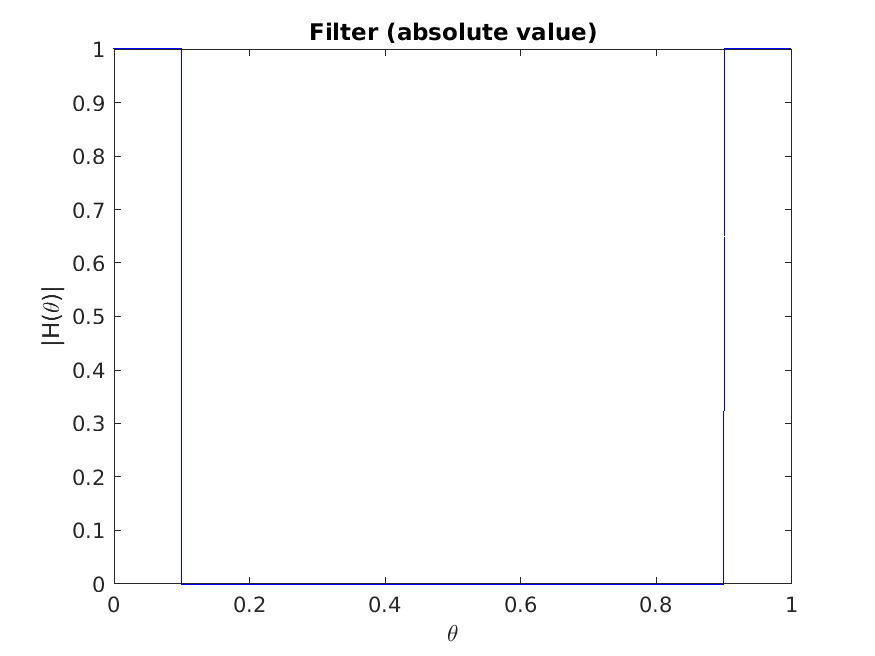
\includegraphics[width=0.7\textwidth]{images/study1/H_hd_th.png}
      \captionof{figure}{Ideal Filter}
    \end{center}
\end{figure}

We will start by calculating the PSD of the filtered signal. If we use formula
\eqref{eq:LTI}, we have:

\begin{equation}\label{eq:R_hd_th}
   R_y(\theta) = R_X(\theta) |H(\theta)|^2 =
   R_X |\text{rect}(\frac{\theta}{\theta_0})|^2 =
   R_X |\text{rect}(\frac{\theta}{0.2})|^2 =
   \begin{cases}
     10 &\quad 0 \le f < 0.1\\
     0 &\quad 0.1 \le f < 0.9\\
     10 &\quad 0.9 \le f < 1\\
   \end{cases}
\end{equation}

\newpage

The resulting graph is:

\begin{figure}[!hp]
    \begin{center}
      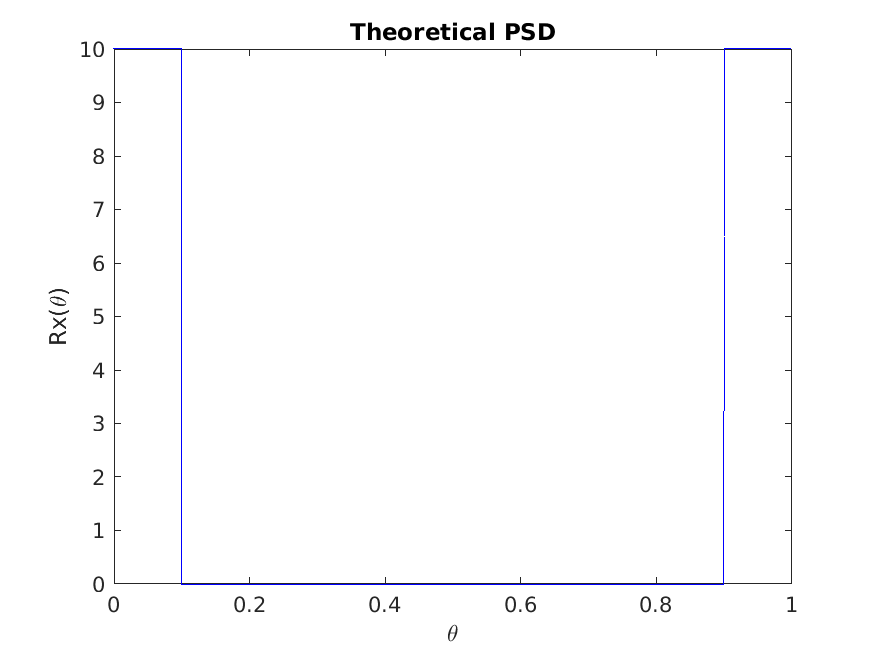
\includegraphics[width=0.58\textwidth]{images/study1/R_hd_th.png}
      \captionof{figure}{Theoretical PSD}
    \end{center}
\end{figure}

To find out the ACF of the signal, we just have to calculate the inverse Fourier
Transform of the PSD:

\begin{equation}\label{eq:r_hd_th}
  \begin{split}
   & \qquad r_y[k] = \mathcal{F}^{-1}\{R_X(\theta)\} =
   \mathcal{F}^{-1}\{R_X|\text{rect}(\frac{\theta}{\theta_0})|^2\} = \\
   & = R_X\cdot\theta_0\cdot \text{sinc}(\theta_0 k) =
   10\cdot0.2\cdot \text{sinc}(0.2 k) = 2\cdot \text{sinc}(0.2 k)
 \end{split}
 \end{equation}

The resulting graph is:

\begin{figure}[!hp]
    \begin{center}
      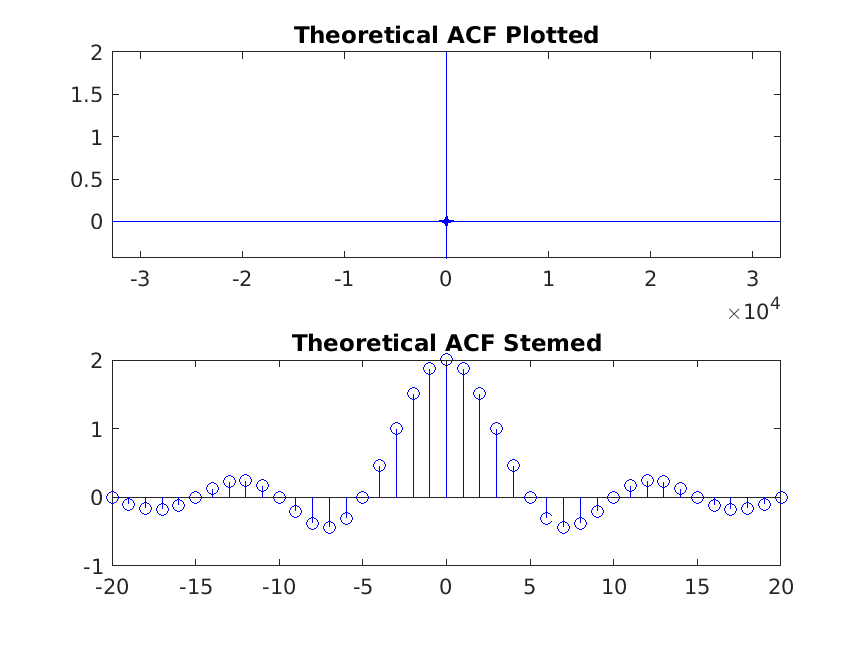
\includegraphics[width=0.58\textwidth]{images/study1/r_hd_th.png}
      \captionof{figure}{Theoretical ACF}
    \end{center}
\end{figure}

\newpage

\subsubsection{Low-degree Filter:}

For the low-degree filter, we will use the filter:

\begin{equation}\label{eq:H_ld_th}
  h[k] = 0.5 \cdot (\delta[k] + \delta[k-1])
\end{equation}

Therefore, in the freuqency domain we have:

\begin{equation}\label{eq:H_ld_th}
  H[\theta] = 0.5\cdot (1+e^{-i 2 \pi \theta})
\end{equation}

We multiply by $0.5$ so that the maximum value of the filter is 1 in stead of
2. \\

This results in the following graph:

\begin{figure}[!hp]
    \begin{center}
      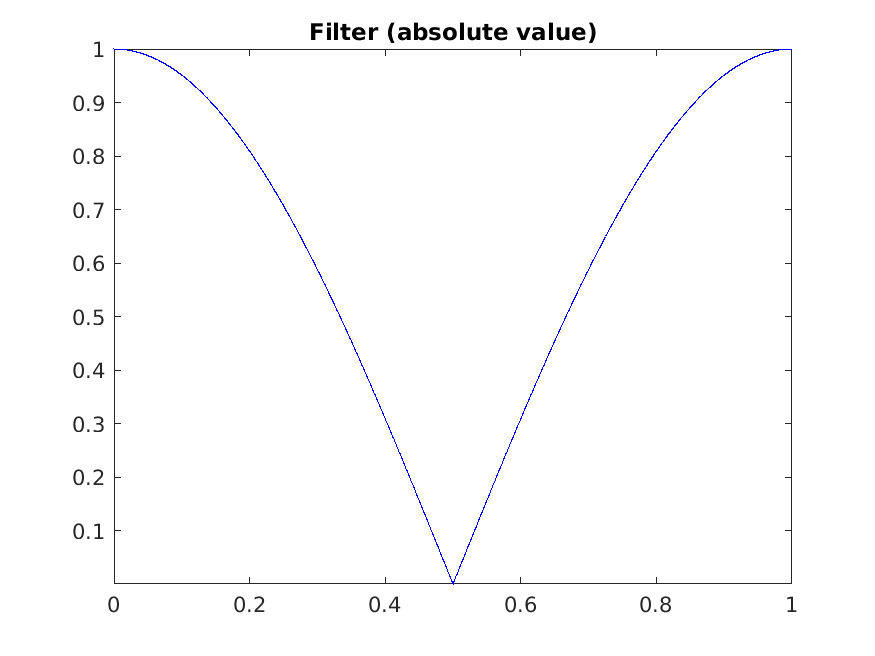
\includegraphics[width=0.8\textwidth]{images/study1/H_ld_th.png}
      \captionof{figure}{Low-Degree Filter}
    \end{center}
\end{figure}

As before, we use formula \eqref{eq:LTI} to get the PSD:

\begin{equation}\label{eq:R_ld_th}
  \begin{split}
   & \qquad\qquad\qquad R_y(\theta) = R_X(\theta) |H(\theta)|^2 = \\
   & = R_X |0.5 \cdot (1 + e^{-i 2 \pi \theta})|^2 =
   R_X \cdot 0.25 |(1 + e^{-i 2 \pi \theta})|^2 = \\
   & = R_X \cdot 0.25 \cdot 2 (1 + \cos(2 \pi \theta) =
   10 \cdot 0.25 \cdot 2 (1 + \cos(2 \pi \theta) = \\
   & \qquad\qquad\qquad\quad = 5 (1 + \cos(2 \pi \theta))
 \end{split}
\end{equation}

\newpage

The graph that formula gives us is:

\begin{figure}[!hp]
    \begin{center}
      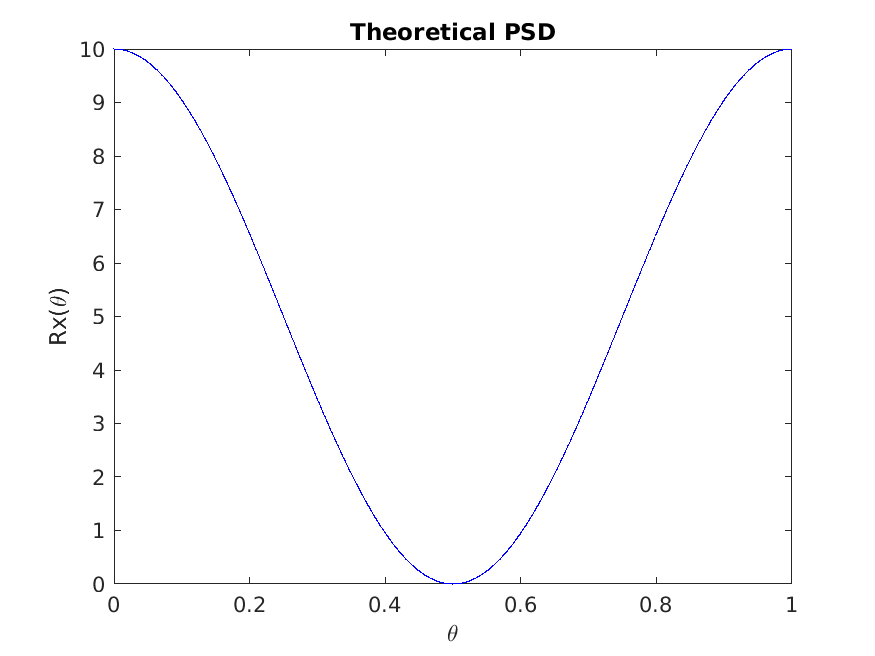
\includegraphics[width=0.55\textwidth]{images/study1/R_ld_th.png}
      \captionof{figure}{Theoretical PSD}
    \end{center}
\end{figure}

Again, to calculate the ACF of the signal, we do the inverse Fourier Transform
of the PSD:

\begin{equation}\label{eq:r_ld_th}
  \begin{split}
     & \qquad r_y[k] = \mathcal{F}^{-1}\{R_X(\theta)\} =
     \mathcal{F}^{-1}\{5 (1 + \cos(2 \pi \theta)\} = \\
     & = 5\delta[k] + 2.5\delta[k-1] + 2.5\delta[k+1] =
     \begin{cases}
         2.5 &\quad k = -1\\
         5 &\quad k = 0\\
         2.5 &\quad k = 1\\
     \end{cases}
 \end{split}
\end{equation}

Therefore, our graph is:

\begin{figure}[!hp]
    \begin{center}
      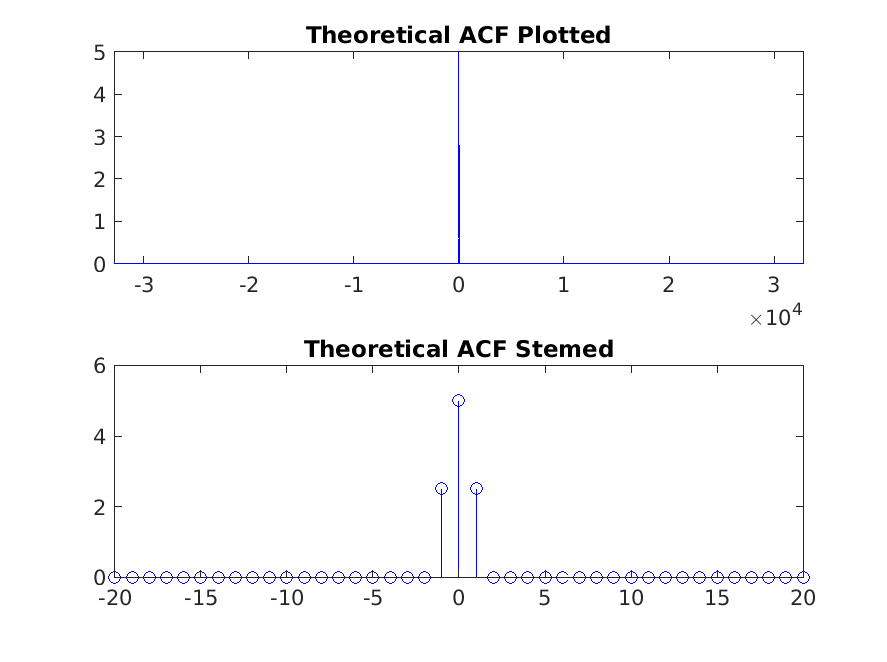
\includegraphics[width=0.55\textwidth]{images/study1/r_ld_th.png}
      \captionof{figure}{Theoretical ACF}
    \end{center}
\end{figure}

\newpage

\subsection{Estimations:}

Let's move on to the estimations. For the ACF we take the Bartlett's ACF
estimate:

\begin{equation}\label{eq:Bartlett}
   \hat{r}_y[k] =
   \begin{cases}
       \displaystyle\sum_{n=0}^{N - |k| - 1} x[n + |k|] x[n] &\quad 0 \le n < N\\
       0 &\quad\text{elsewhere}\\
   \end{cases}
\end{equation}

For the PSD we can just do the Fourier Transform MatLab function \textit{fft(x)}.

\subsubsection{High-degree Filter:}

For the ideal filter, the estimation for the ACF is the following:

\begin{figure}[!hp]
    \begin{center}
      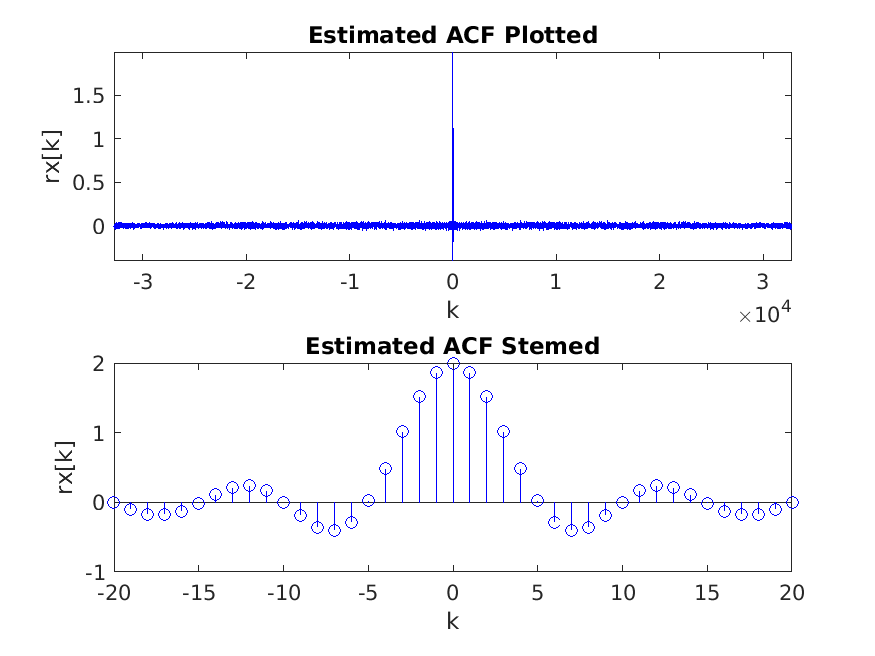
\includegraphics[width=0.8\textwidth]{images/study1/r_hd_es.png}
      \captionof{figure}{Estimated ACF}
    \end{center}
\end{figure}

As we can see, it is very close to the the theoretical estimation. The plotted
graph is slightly more noisy, but the stemed graph is practically the same.

\newpage

\begin{figure}[!hp]
    \begin{center}
      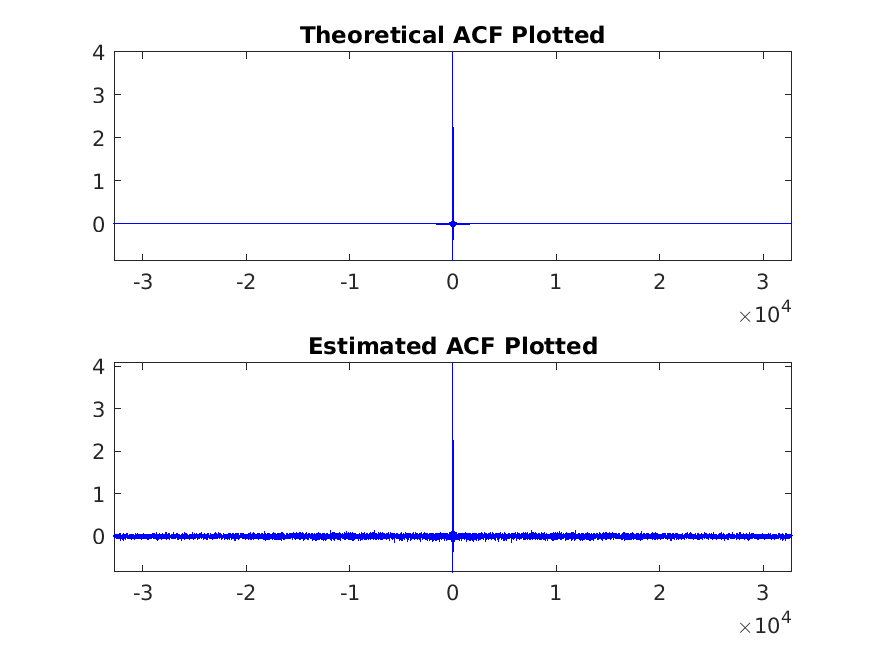
\includegraphics[width=0.7\textwidth]{images/study1/comp_r_hd_plot.png}
      \captionof{figure}{Compared ACF}
    \end{center}
\end{figure}

\begin{figure}[!hp]
    \begin{center}
      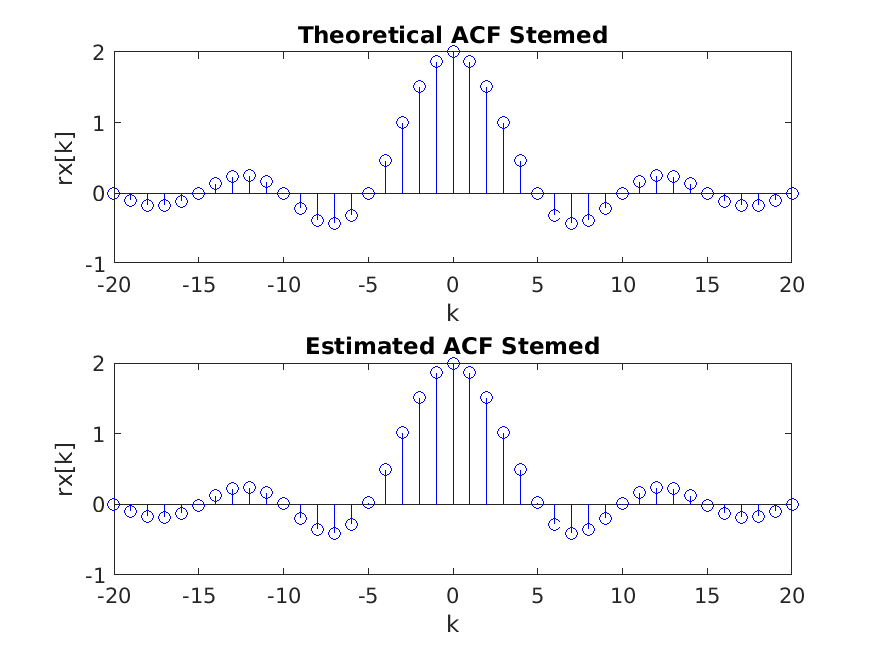
\includegraphics[width=0.7\textwidth]{images/study1/comp_r_hd_stem.png}
      \captionof{figure}{Compared ACF}
    \end{center}
\end{figure}

\newpage

The PSD graph resulting from the Fourier Transform of the above is:

\begin{figure}[!hp]
    \begin{center}
      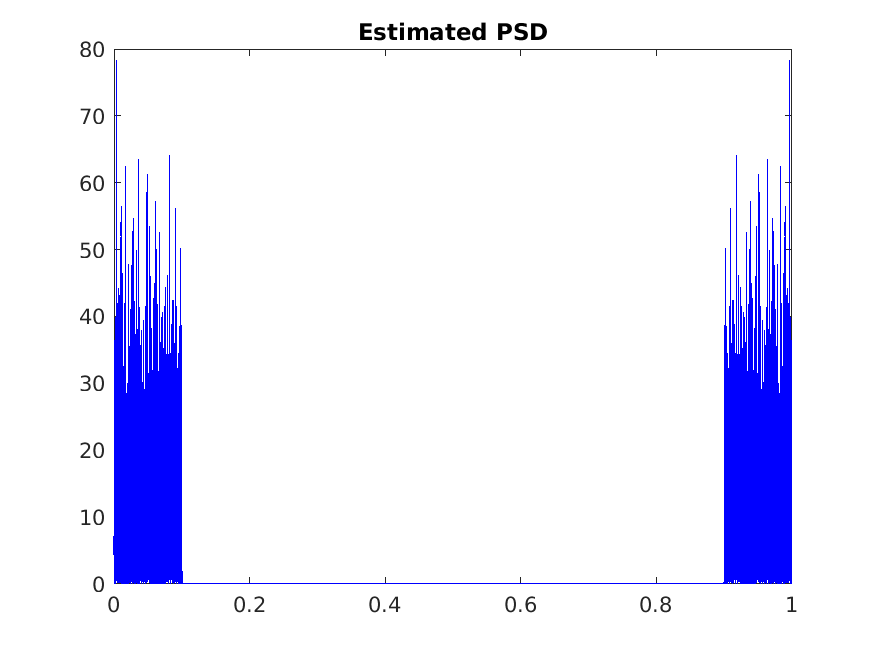
\includegraphics[width=0.65\textwidth]{images/study1/R_hd_es.png}
      \captionof{figure}{Estimated PSD}
    \end{center}
\end{figure}

On plain sight, it looks very different from the theoretical PSD graph, but
because it has a lot of noise. During study 2 we will see that the values once
we average or smooth the PSD are the same as the theoretical analysis.

\begin{figure}[!hp]
    \begin{center}
      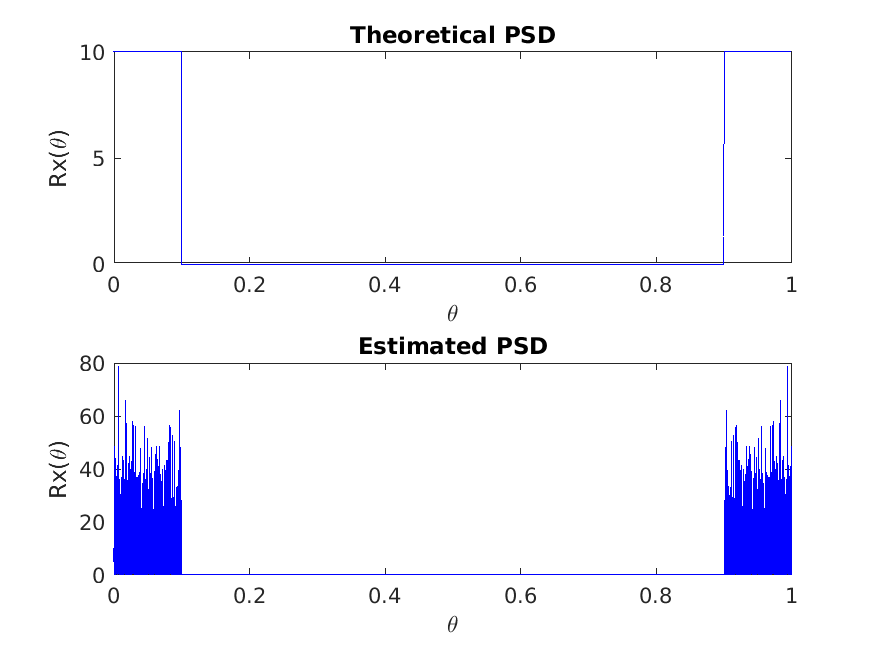
\includegraphics[width=0.65\textwidth]{images/study1/comp_R_hd.png}
      \captionof{figure}{Compared PSD}
    \end{center}
\end{figure}

\newpage

\subsubsection{Low-degree Filter:}

For the simple filter, the estimation for the ACF results in this graph:

\begin{figure}[!hp]
    \begin{center}
      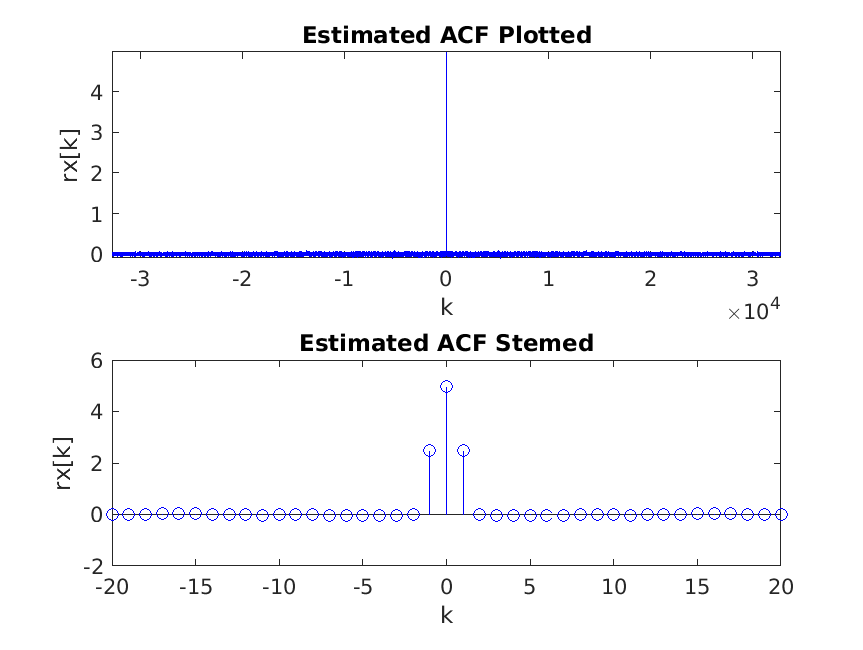
\includegraphics[width=0.8\textwidth]{images/study1/r_ld_es.png}
      \captionof{figure}{Estimated ACF}
    \end{center}
\end{figure}

Again, it is very close to the the theoretical estimation. Once more, we can see
that the plotted graph is ticker in the x-axis, and the stemmed graph has values
slightly under 0, which we didn't have in the theoretical analysis, but it
is practicacly imperceptible.

\newpage

\begin{figure}[!hp]
    \begin{center}
      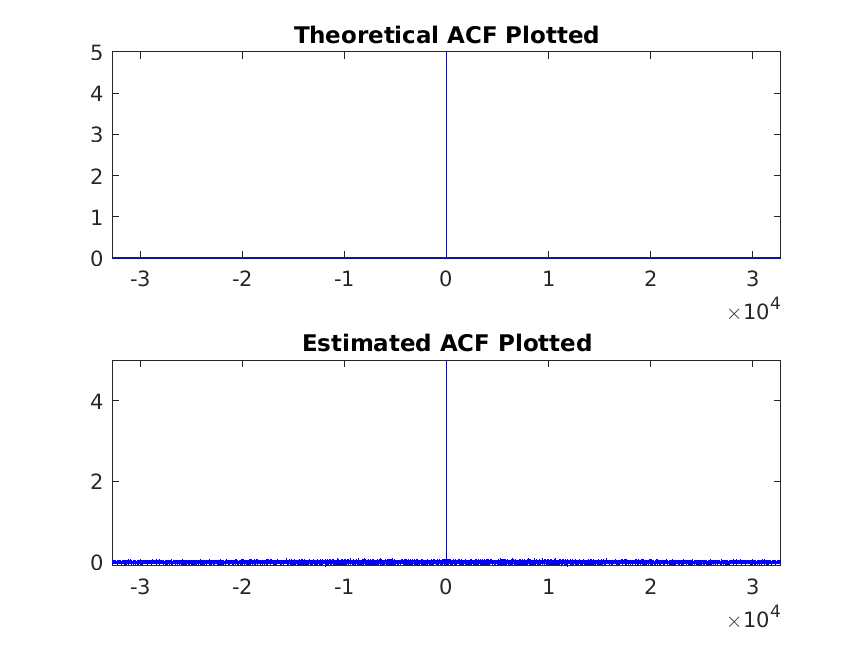
\includegraphics[width=0.7\textwidth]{images/study1/comp_r_ld_plot.png}
      \captionof{figure}{Compared ACF}
    \end{center}
\end{figure}

\begin{figure}[!hp]
    \begin{center}
      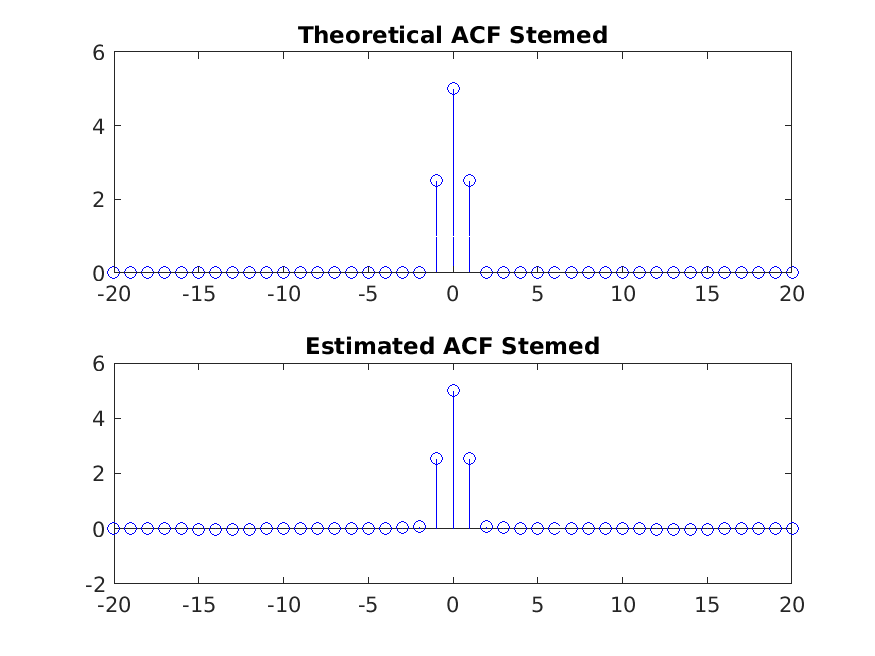
\includegraphics[width=0.7\textwidth]{images/study1/comp_r_ld_stem.png}
      \captionof{figure}{Compared ACF}
    \end{center}
\end{figure}

\newpage

The PSD graph that we get from the Fourier Transform of the ACF is:

\begin{figure}[!hp]
    \begin{center}
      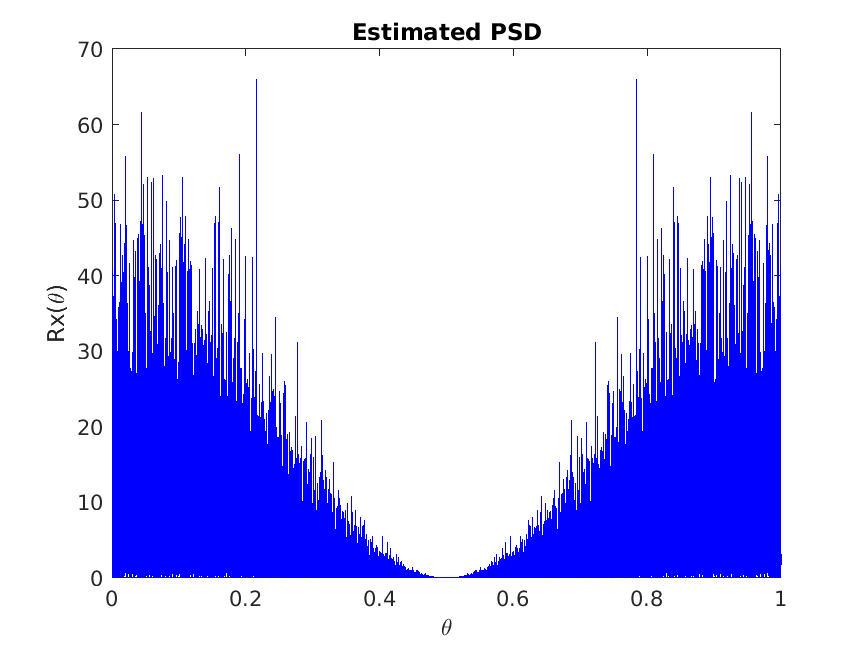
\includegraphics[width=0.65\textwidth]{images/study1/R_ld_es.png}
      \captionof{figure}{Estimated PSD}
    \end{center}
\end{figure}

Here we have the same case as before, now we have a pointy and noisy draft of
the PSD that, in the next study, will start to resemble more to the theoretical
PSD.

\begin{figure}[!hp]
    \begin{center}
      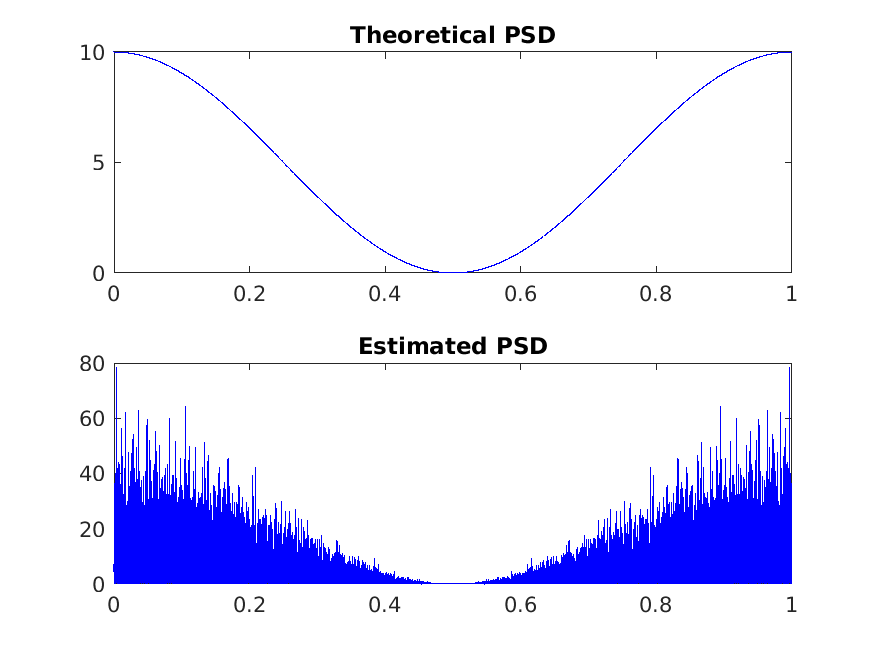
\includegraphics[width=0.65\textwidth]{images/study1/comp_R_ld.png}
      \captionof{figure}{Compared PSD}
    \end{center}
\end{figure}

\newpage

\section{Study 2:}

\subsection{Theoretical Background:}

In this second study, the aim is to improve the estimates done in the first
study. We will use all the graphs we got from study 1, and improve them in two
different ways:

\begin{itemize}
  \item \textbf{Windows:}
  For the windowing technique, we will take five different windows:

  \begin{figure}[!hp]
      \begin{center}
        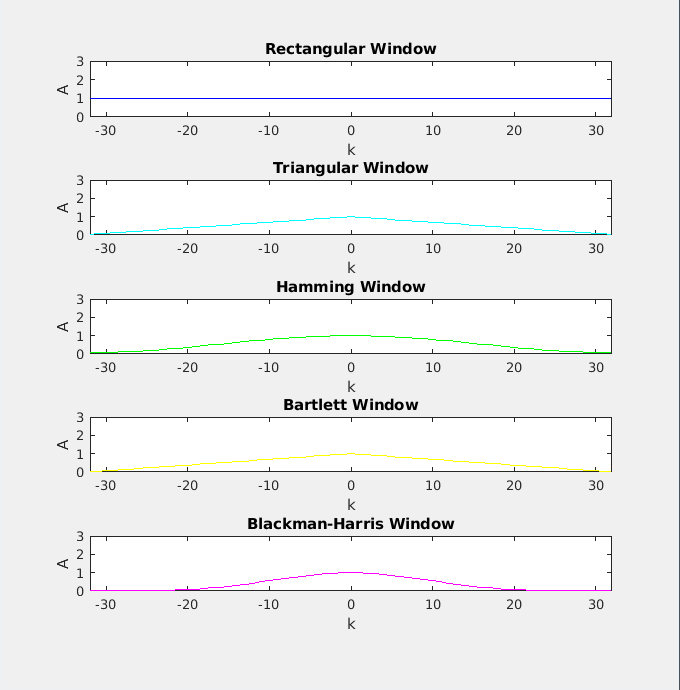
\includegraphics[width=0.6\textwidth]{images/study2/windows2.png}
      \captionof{figure}{Compared PSD}
      \end{center}
  \end{figure}

  We will pad them with zeros and then use them to window our estimated ACF to
  smooth our graphs. We will get the PSD with the Fourier Transform again.

  \item \textbf{Averaging:}
  The basis of this technique is spliting the signal is several parts,
  estimating each one of them and then averaging all the results. This allowes
  us to reduce the variance and the pointy look of the PSD. We follow the
  following formula:

  \begin{equation}\label{eq:Averaging}
    R_{X_{Av}}[\theta] = \displaystyle\frac{1}{K} \displaystyle\sum_{k=1}^{K} \hat{R}_{X,k}[\theta]
  \end{equation}

  We will use three different values to compare them, $2^4$, $2^6$ and $2^8$.
  Once again, we will apply it to the ACF and then switch to frequency domain.

\end{itemize}

\newpage

\subsection{Smoothing:}

We will start with the window smoothing.

\subsubsection{High-degree Filter:}

Here we have the ACF:

\begin{figure}[!hp]
    \begin{center}
      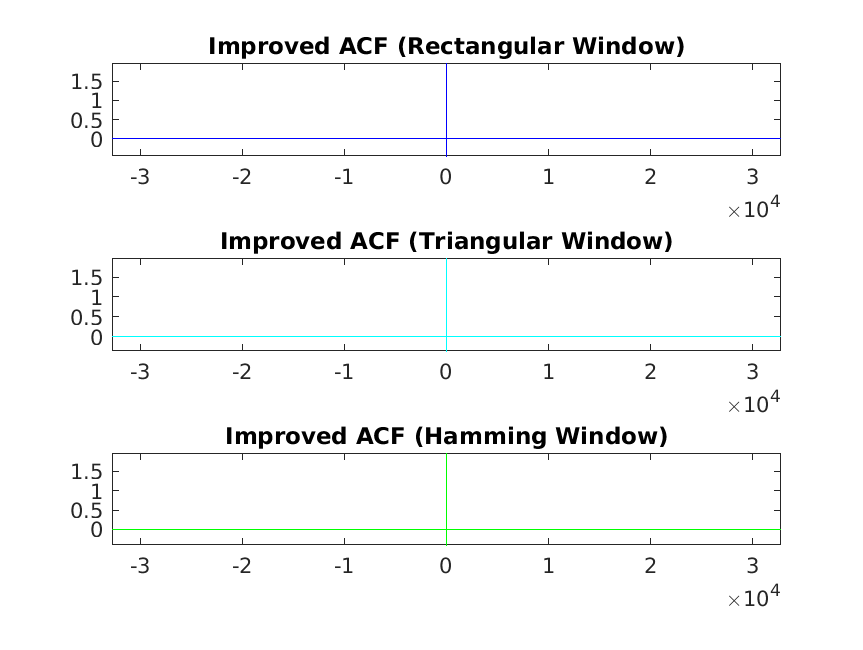
\includegraphics[width=0.6\textwidth]{images/study2/acf_hd_plot1.png}
    \end{center}
\end{figure}

\begin{figure}[!hp]
    \begin{center}
      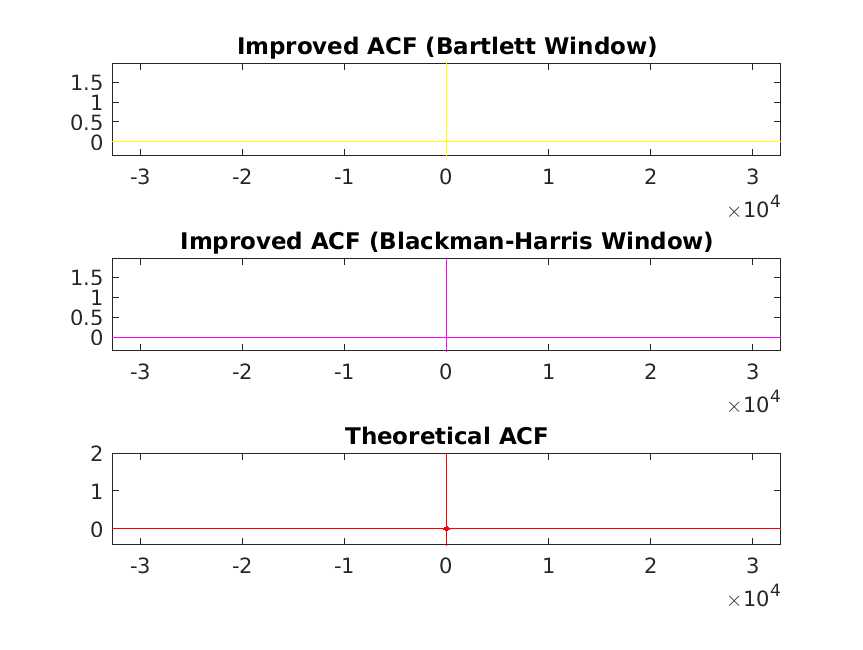
\includegraphics[width=0.6\textwidth]{images/study2/acf_hd_plot2.png}
      \captionof{figure}{Smoothed ACF}
    \end{center}
\end{figure}

As we can see, the noisy-look we had before has dissappeared, and now the
estimated ACF looks more like the theoretical ACF.

\newpage

\begin{figure}[!hp]
    \begin{center}
      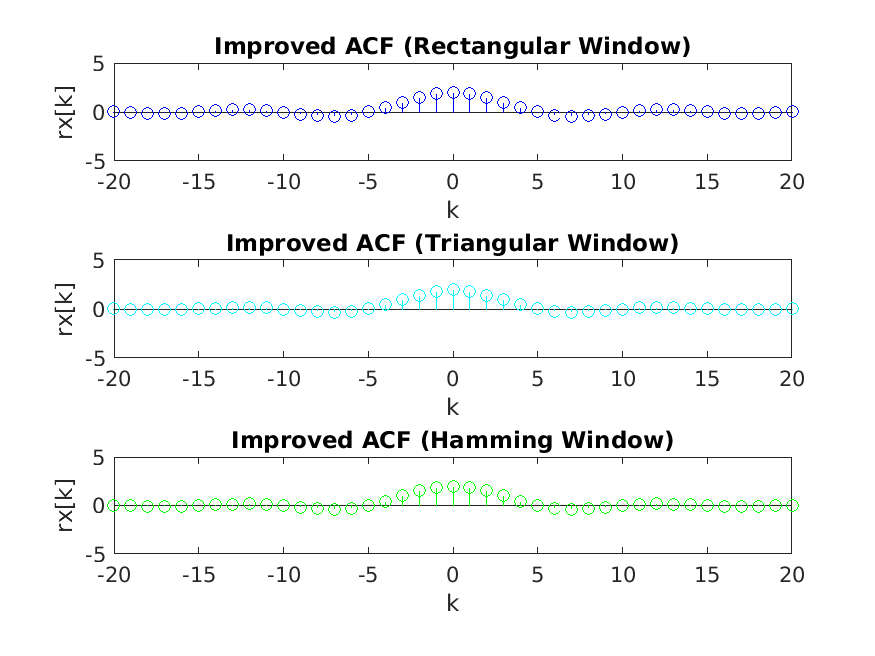
\includegraphics[width=0.6\textwidth]{images/study2/acf_hd_stem1.png}
    \end{center}
\end{figure}

\begin{figure}[!hp]
    \begin{center}
      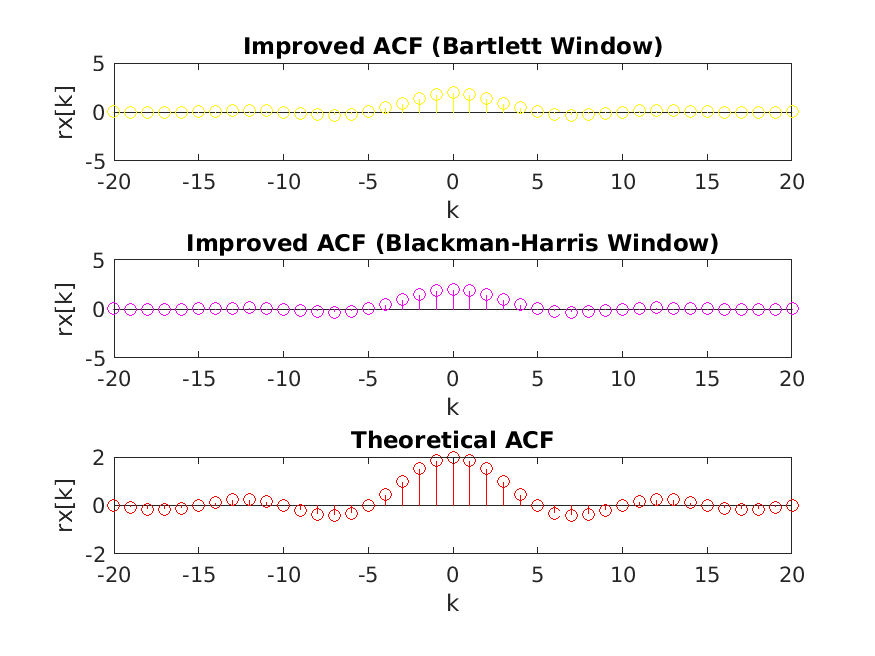
\includegraphics[width=0.6\textwidth]{images/study2/acf_hd_stem2.png}
      \captionof{figure}{Smoothed ACF}
    \end{center}
\end{figure}

Here there is not much difference, since the estimated graph close up was
almost the same as the theoretical graph.

\newpage

Here we have the PSD:

\begin{figure}[!hp]
    \begin{center}
      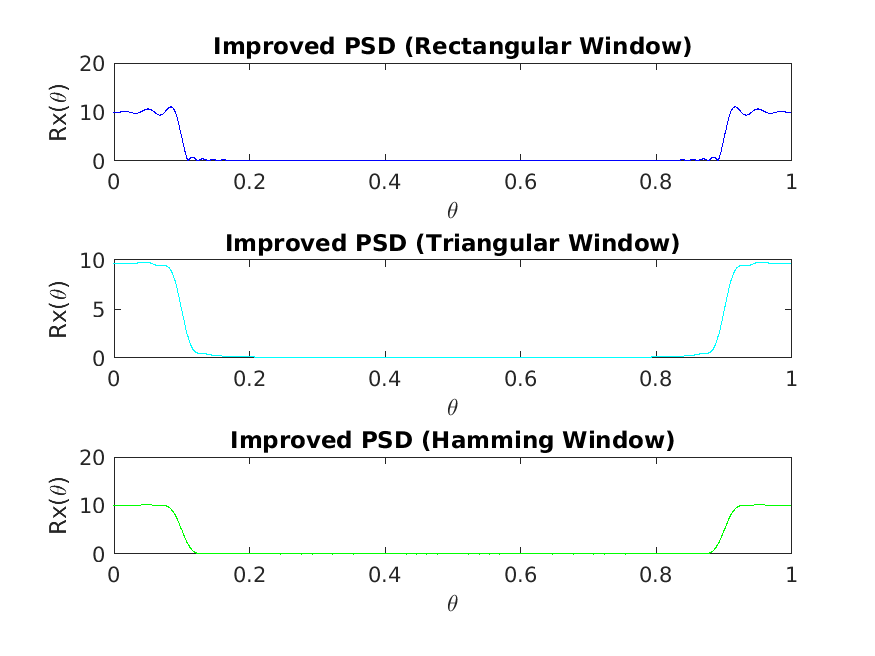
\includegraphics[width=0.6\textwidth]{images/study2/psd_hd_window1.png}
    \end{center}
\end{figure}

\begin{figure}[!hp]
    \begin{center}
      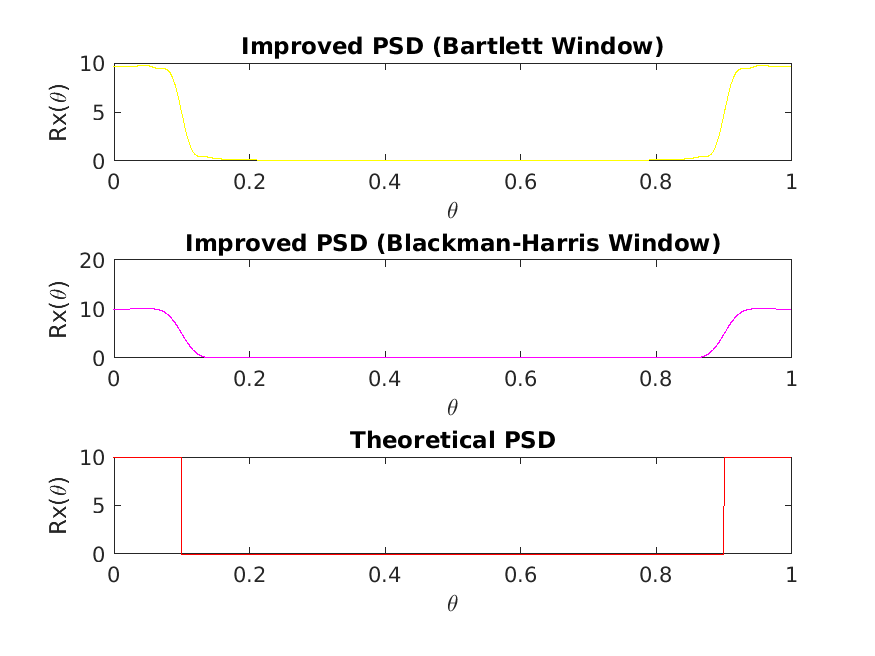
\includegraphics[width=0.6\textwidth]{images/study2/psd_hd_window2.png}
      \captionof{figure}{Smoothed PSD}
    \end{center}
\end{figure}

The high variance that we had before is not there anymore, but the edges of the
curve still look rounder than they should, and the step is not abrupt enough.

\newpage

\subsubsection{Low-degree Filter:}

Here we have the ACF:

\begin{figure}[!hp]
    \begin{center}
      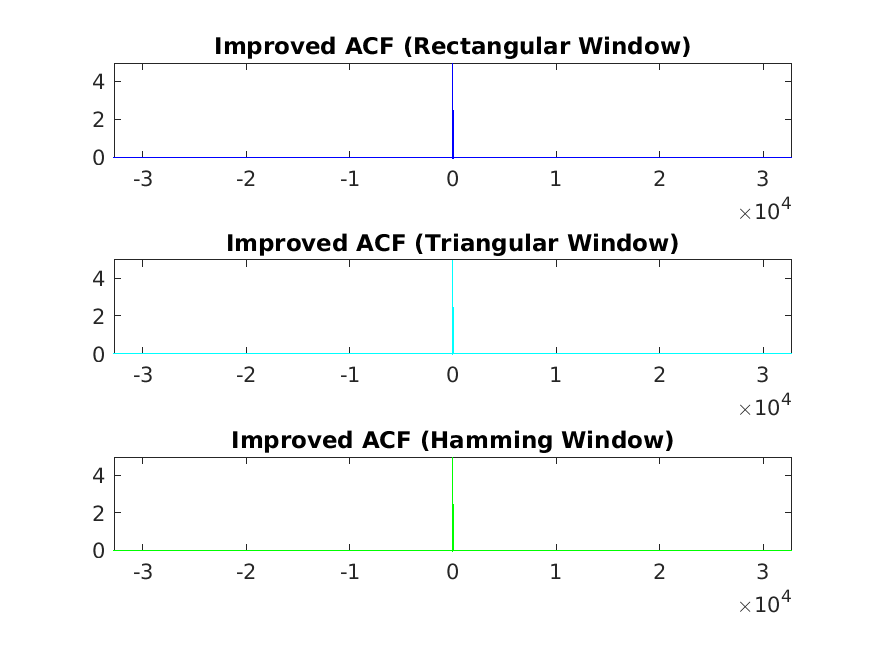
\includegraphics[width=0.6\textwidth]{images/study2/acf_ld_plot1.png}
    \end{center}
\end{figure}

\begin{figure}[!hp]
    \begin{center}
      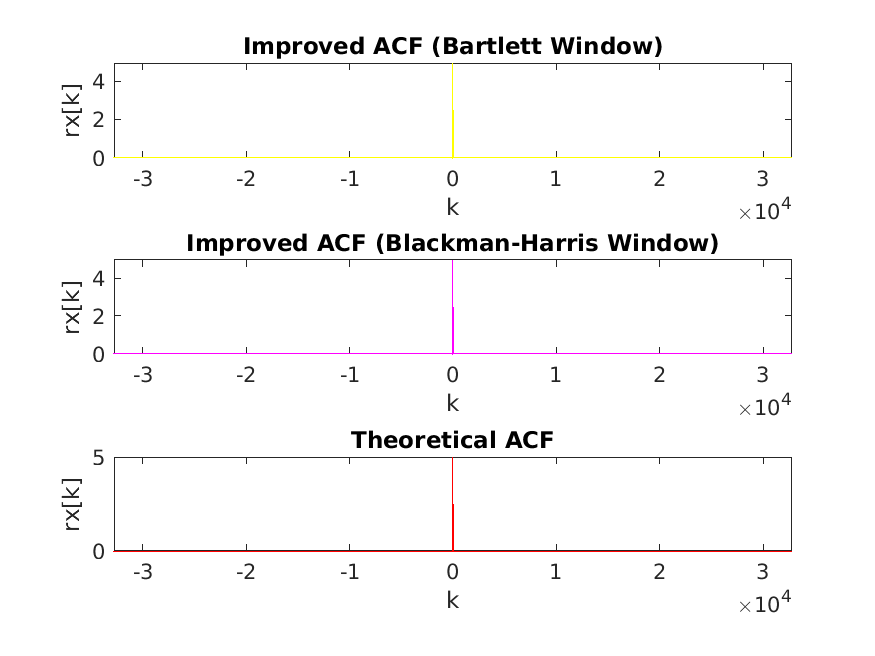
\includegraphics[width=0.6\textwidth]{images/study2/acf_ld_plot2.png}
      \captionof{figure}{Smoothed ACF}
    \end{center}
\end{figure}

This is the same case as the high-degree filter, now the graph has less variance
in respect of the x-axis.

\newpage

\begin{figure}[!hp]
    \begin{center}
      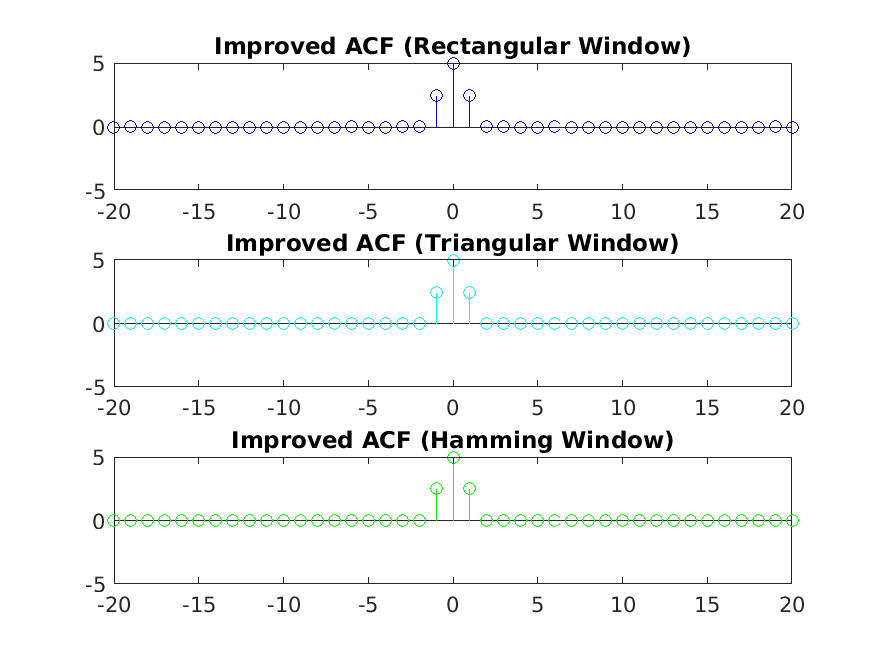
\includegraphics[width=0.6\textwidth]{images/study2/acf_ld_stem1.png}
    \end{center}
\end{figure}

\begin{figure}[!hp]
    \begin{center}
      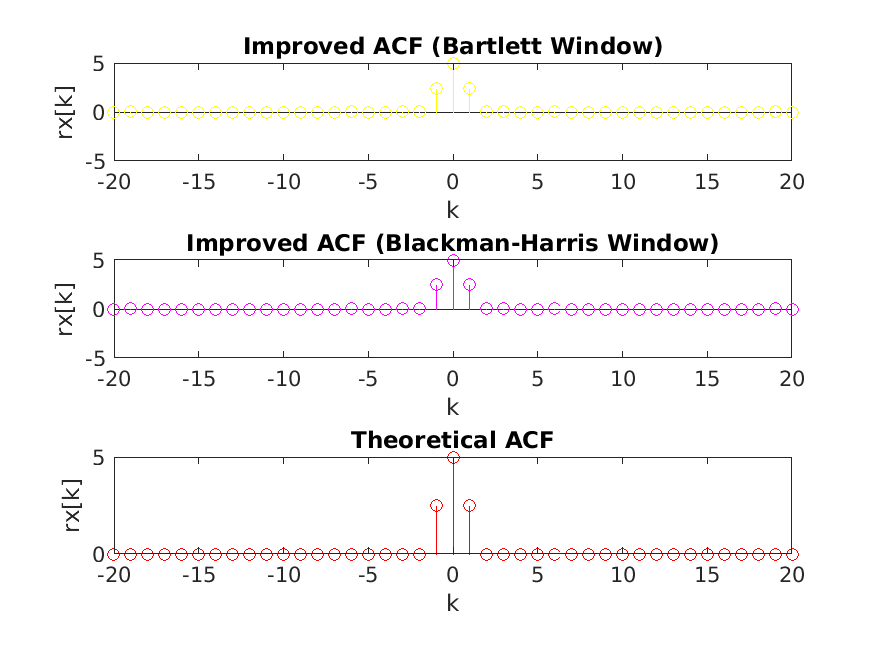
\includegraphics[width=0.6\textwidth]{images/study2/acf_ld_stem2.png}
      \captionof{figure}{Smoothed ACF}
    \end{center}
\end{figure}

Here, again, there is not much difference, our estimation was very accurate
already.

\newpage

Here we have the PSD:

\begin{figure}[!hp]
    \begin{center}
      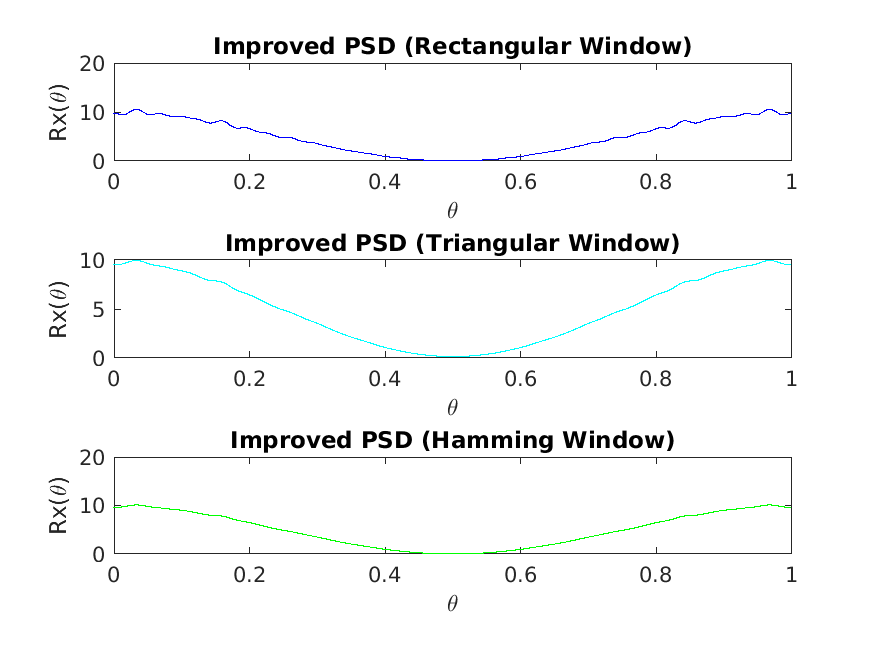
\includegraphics[width=0.6\textwidth]{images/study2/psd_ld_window1.png}
    \end{center}
\end{figure}

\begin{figure}[!hp]
    \begin{center}
      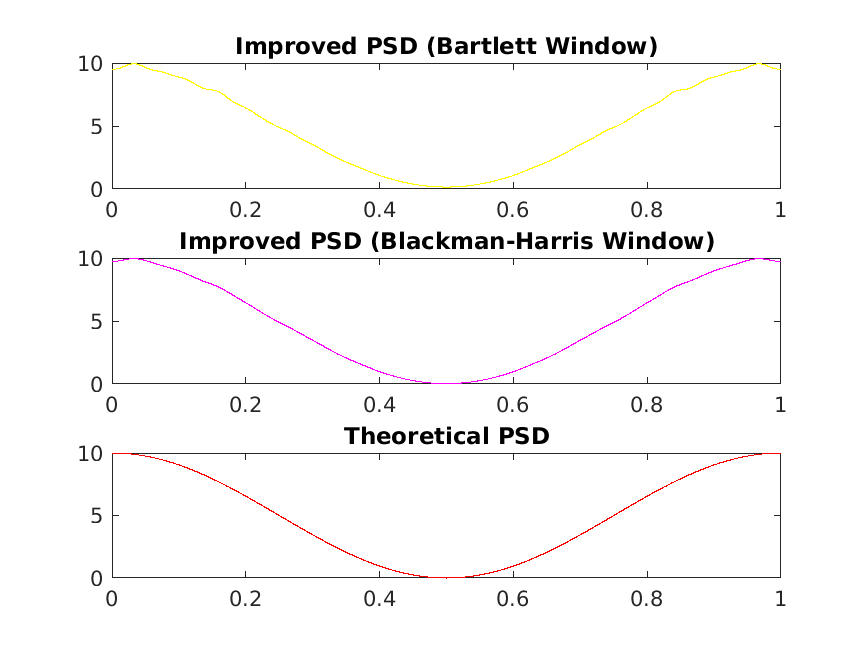
\includegraphics[width=0.6\textwidth]{images/study2/psd_ld_window2.png}
      \captionof{figure}{Smoothed PSD}
    \end{center}
\end{figure}

In this PSD we don't have sharp edges, therefore the improvements fit better
the theoretical graph than how they did for they high-degree filter. Now we
only have a bit of variance, specially with the Rectangular and Triangular
window, but with the Blackman-Harris window, the improvement is almost perfect.

\newpage

\subsection{Averaging:}

Now let's move on to the improvements through averaging:

\subsubsection{High-degree Filter:}

\begin{figure}[!hp]
    \begin{center}
      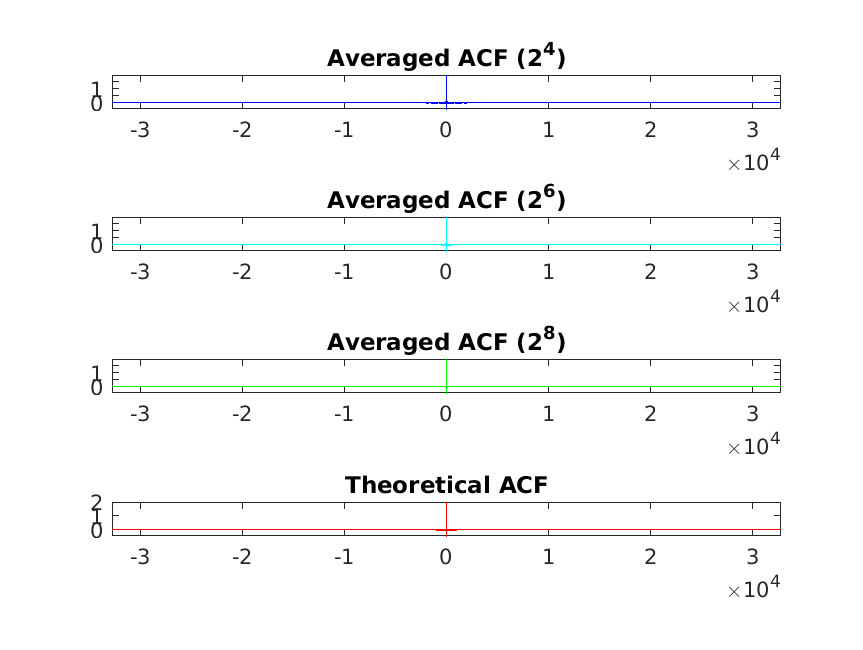
\includegraphics[width=0.58\textwidth]{images/study2/acf_hd_aver_plot.png}
      \captionof{figure}{Averaged ACF}
    \end{center}
\end{figure}

\begin{figure}[!hp]
    \begin{center}
      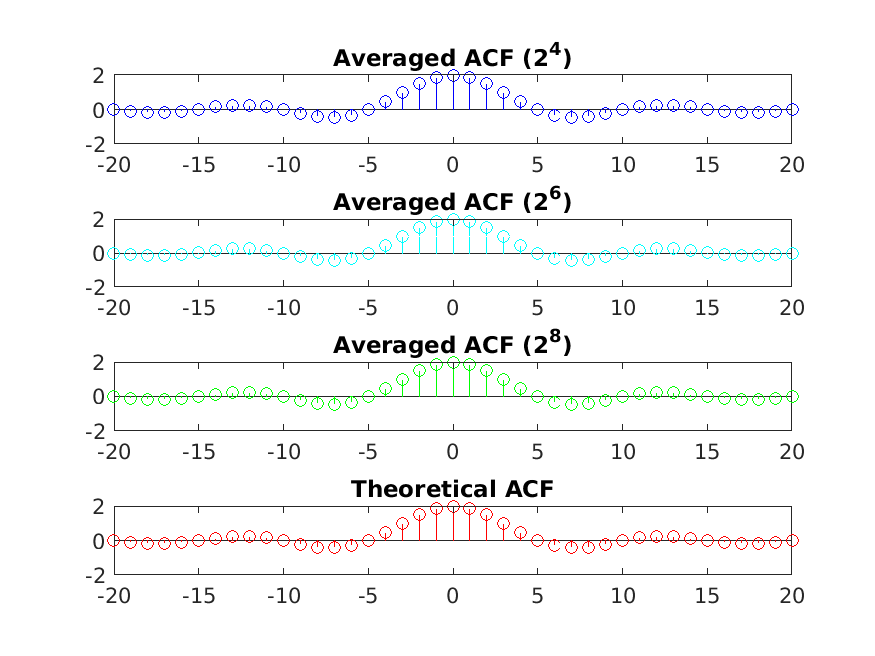
\includegraphics[width=0.58\textwidth]{images/study2/acf_hd_aver_stem.png}
      \captionof{figure}{Averaged ACF}
    \end{center}
\end{figure}

We have the same situations as with smoothing: the ACF estimation was very
accurate already, so we can not see big changes. Nevertheless, we can notice
how in the plotted graph, the noise around 0 decreases as we have higher values
for the averaging, since it becomes more accurate.

\newpage

\begin{figure}[!hp]
    \begin{center}
      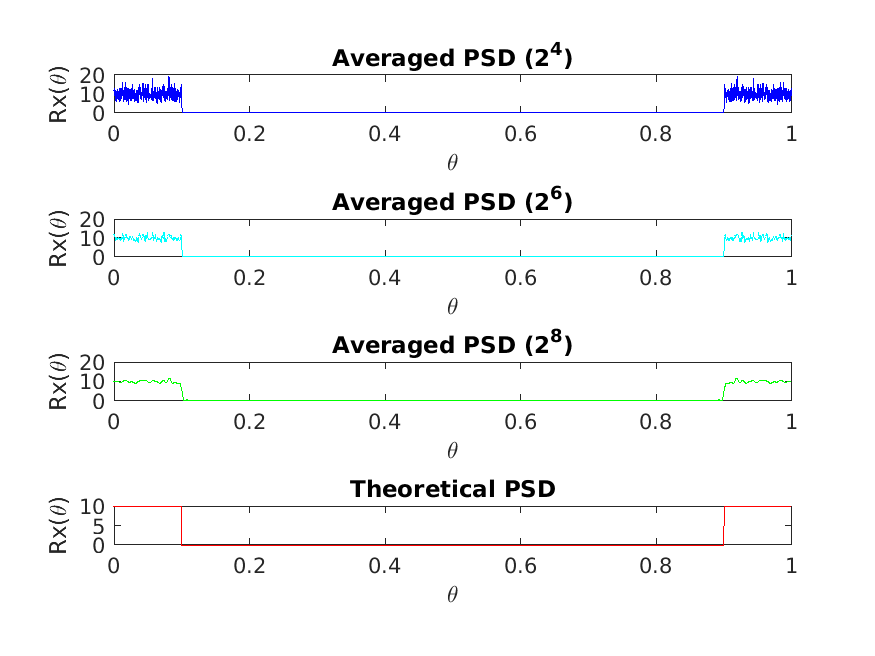
\includegraphics[width=0.8\textwidth]{images/study2/psd_hd_aver.png}
      \captionof{figure}{Averaged PSD}
    \end{center}
\end{figure}

Here we can clearly see the changes. The lower the value, the more it still
looks like the raw periodogram. Nevertheless, we only go up to $2^8$ because if
the averaging values get near $2^{16}$, that is, our number of samples, the
averaged periodogram becomes distorted. \\

This improvement is better for the PSD since it respects the sharp edges of the
rectangle function, and therefore makes the estimation fit better the
theoretical graph.

\newpage

\subsubsection{Low-degree Filter:}

\begin{figure}[!hp]
    \begin{center}
      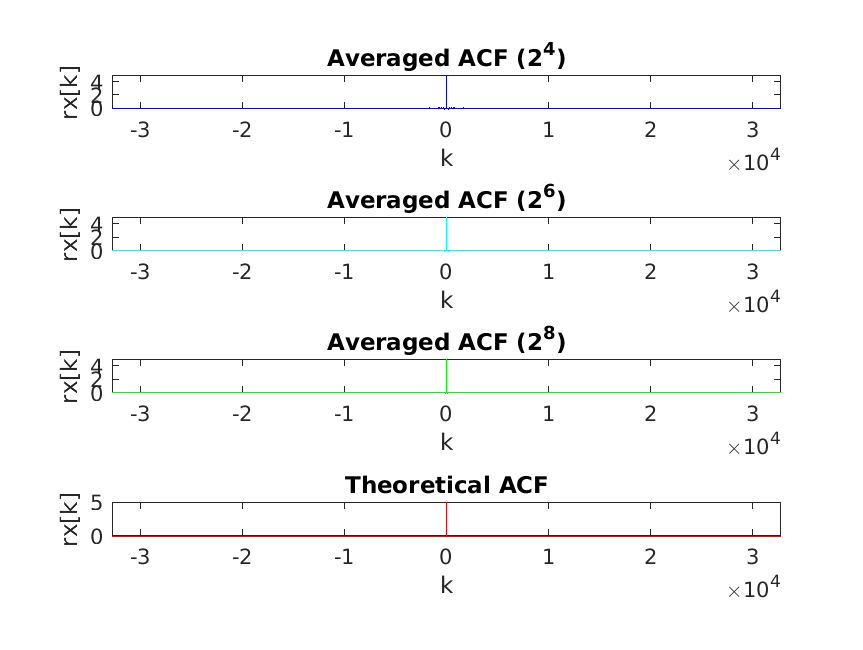
\includegraphics[width=0.58\textwidth]{images/study2/acf_ld_aver_plot.png}
      \captionof{figure}{Averaged ACF}
    \end{center}
\end{figure}

\begin{figure}[!hp]
    \begin{center}
      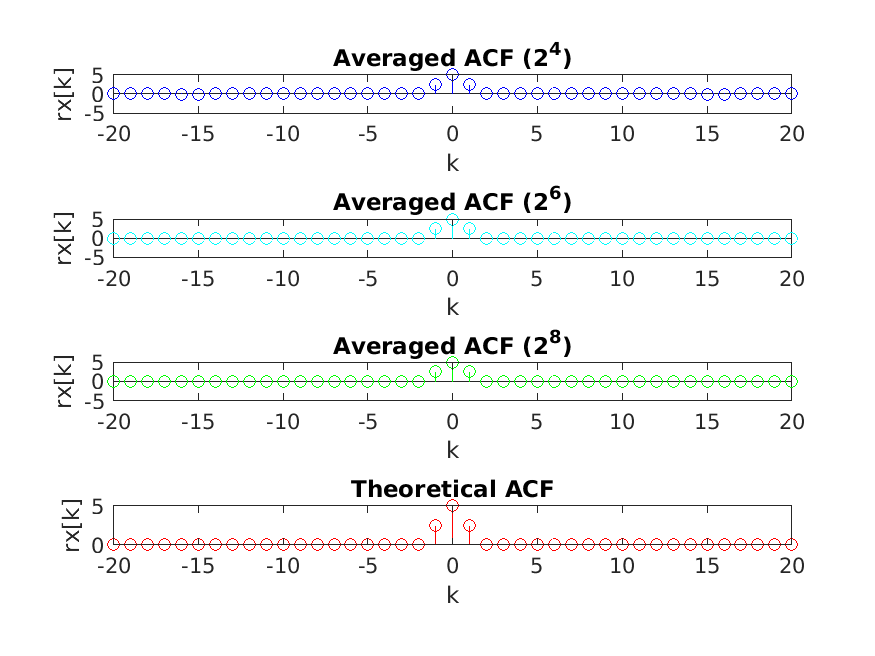
\includegraphics[width=0.58\textwidth]{images/study2/acf_ld_aver_stem.png}
      \captionof{figure}{Averaged ACF}
    \end{center}
\end{figure}

Again, we can notice how in the plotted graph, the noise around 0 decreases
as we have higher values for the averaging, but it decreases at a higher rate
than it did with the high-degree filter.

\newpage

\begin{figure}[!hp]
    \begin{center}
      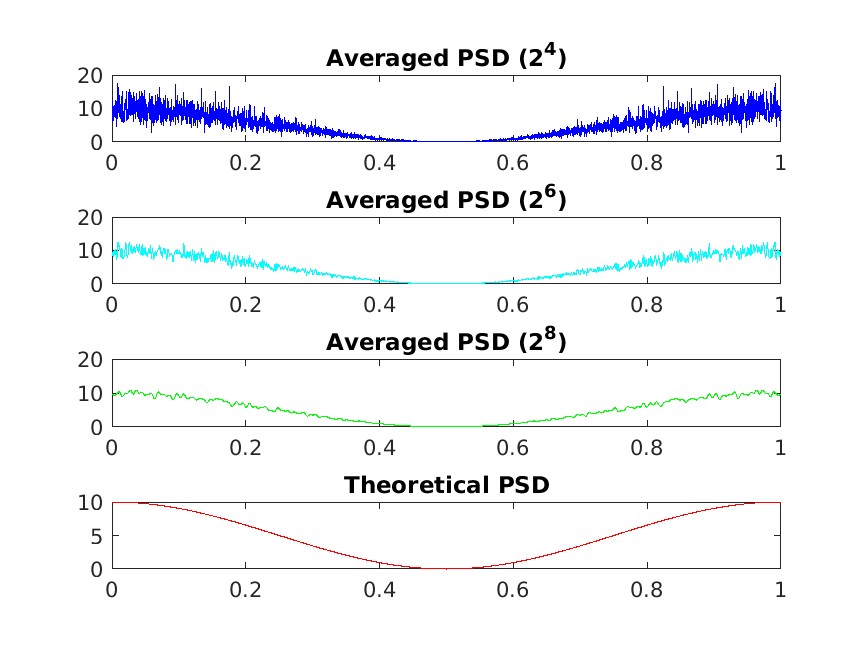
\includegraphics[width=0.8\textwidth]{images/study2/psd_ld_aver.png}
      \captionof{figure}{Averaged PSD}
    \end{center}
\end{figure}

The improved graph is good, now we don't have that much variance and the
highest value is really similar to the theoretical graph, but the improvements
we did with windows were more accurate and less "irregular". \\

Therefore, if we have a smooth and curvy graph, it is better to use windows
because it will be more accurate, but if we have a graph with sharp edges,
working with windows might make them appear smoother than we would like to,
so it is better to work with averaging because even if it looks a bit noisy
still, the shape in the end will be more similar to the theoretical one.

\newpage

\section{Study 3:}

\subsection{Theoretical Background:}

We have the three following systems:

\begin{itemize}

\item A squarer:

\begin{equation}\label{eq:Squarer}
  Y[n] = X^2[n]
\end{equation}

\item A half-wave rectifier:

\begin{equation}\label{eq:HW}
  Y[n] =
    \begin{cases}
        X[n], &\quad n: X[n] > 0\\
        0,    &\quad n: X[n] \leq 0
    \end{cases}
\end{equation}

\item An AM-SC modulator:

\begin{equation}\label{eq:AMSC}
  Y[n] = X[n]\cos(\omega_{carrier} n)
\end{equation}

\end{itemize}

Each one of those is a non-LTI system, that is, even if out input signal is
Gaussian and linear, the output doesn't have to be (and probably won't be)
Gaussian and linear. \\

We will use White Gaussian Noise and our high-degree low-pass filter to analyze
how these three systems react to out input, and to see how we can spot if a
system is LTI or non-LTI.\\

None of them following a linear equation means that we cannot use our regular
formula \eqref{eq:LTI} to calculate the PSD. We have to use special formulas
that we can find in the course book. Let's move on to the special calculations
for each system.

\newpage

\subsection{Theoretical Analysis:}

\subsubsection{Squarer:}

For the squarer, we can check on the book that the ACF formula is:

\begin{equation}\label{eq:r_sq}
  r_Y[k] = 2r_X^2[k] + r_X^2[0]
\end{equation}

To calculate the PSD, we just have to swith to frequency domain:

\begin{equation}\label{eq:R_sq}
  \begin{split}
    & \qquad R_Y[\theta] = \mathcal{F}\{r_Y[k]\} = \\
    & = 2 (R_X \ast R_X)[\theta] +
    r_X^2[0]\displaystyle\sum_{m}\delta(\theta) = \\
    & = \displaystyle\frac{1}{4} r_X^2[0]\delta(\theta) +
    4 R_X \text{triangle}(\frac{\theta}{2 BW})
  \end{split}
\end{equation}

The resulting graph is:

\begin{figure}[!hp]
    \begin{center}
      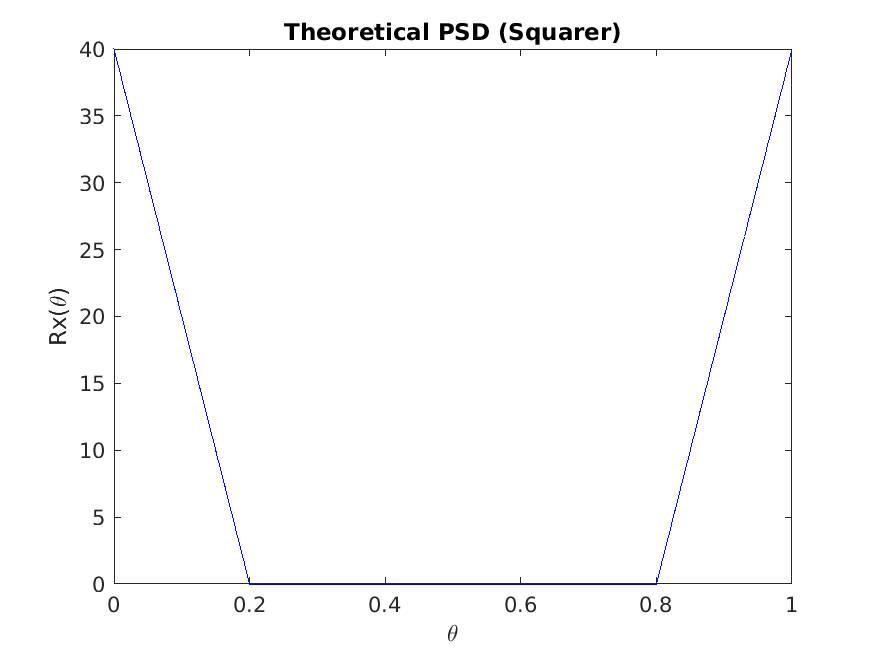
\includegraphics[width=0.8\textwidth]{images/study3/R_th_sq.png}
      \captionof{figure}{Theoretical PSD}
    \end{center}
\end{figure}

\newpage

\subsubsection{Half-Wave Rectifier:}

For the half-wave rectifier, we can check on the book that the ACF formula is:

\begin{equation}\label{eq:r_hw}
  r_Y[k] = \frac{r_X[0]}{2\pi}
  +\frac{r_X[k]}{4}+\frac{r_X^2[k]}{4\pi r_X[0]}
\end{equation}

We switch to the frequency domain:

\begin{equation}\label{eq:R_hw}
  \begin{split}
  & \qquad\qquad\qquad R_Y[\theta] = \mathcal{F}\{r_Y[k]\} = \\
  & = R_Y[\theta] = \displaystyle\frac{r_X[0]}{2\pi}\delta[\theta] +
  \displaystyle\frac{R_X[\theta]}{4} +
  \frac{(R_X\ast R_X)[\theta]}{4\pi r_X[0]} = \\
  & = \displaystyle\frac{R_X}{4\pi}\delta[\theta] +
  \displaystyle\frac{R_X}{4\pi} \text{triangle}[\frac{\theta}{2 BW}] +
  \frac{R_X}{4}\text{rect}[\frac{\theta}{2 BW}]
  \end{split}
\end{equation}

The resulting graph from applying that equation is:

\begin{figure}[!hp]
    \begin{center}
      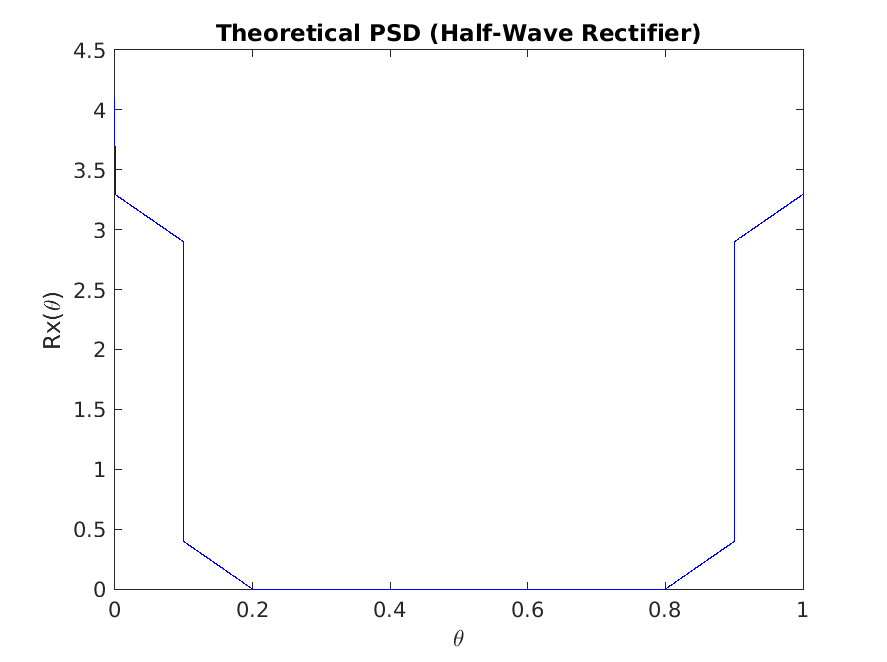
\includegraphics[width=0.8\textwidth]{images/study3/R_th_hw.png}
      \captionof{figure}{Theoretical PSD}
    \end{center}
\end{figure}

\newpage

\subsubsection{AM-SC Modulator:}

For the AM-SC Modulator, we are multiplying our signal by a carrier. Our
carrier will have aplitude $A = 1$ and frequency $f_{carrier} = 0.25$.

\begin{equation}\label{eq:carrier}
  Carrier[k] = \cos(\omega_{carrier} k)
\end{equation}

We can check on the book that the ACF formula is:

\begin{equation}\label{eq:r_am}
  r_Y[k] = \frac{A^2}{2}\cos(2\pi f_{carrier} k) =
  \frac{A^2}{2}\cos(\omega_{carrier} k)
\end{equation}

We switch to the frequency domain:

\begin{equation}\label{eq:R_am}
  \begin{split}
  & \qquad\qquad\qquad R_Y[\theta] = \mathcal{F}\{r_Y[k]\} = \\
  & =\displaystyle\frac{R_X}{4}(\text{rect}[\frac{\theta - f_{carrier}}{BW}] +
  \text{rect}[\frac{\theta + f_{carrier}}{BW}])
  \end{split}
\end{equation}

The resulting graph from applying that equation is:

\begin{figure}[!hp]
    \begin{center}
      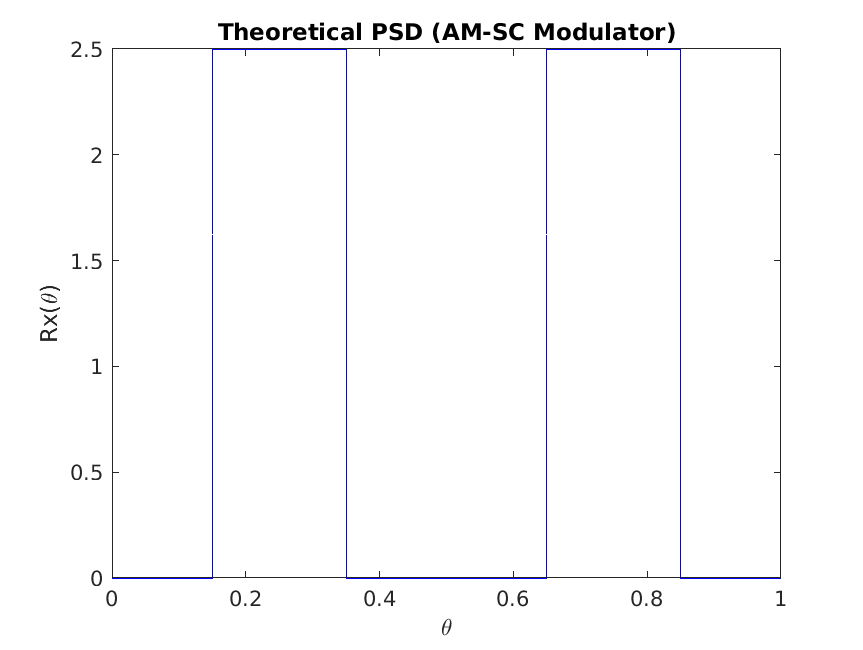
\includegraphics[width=0.8\textwidth]{images/study3/R_th_am.png}
      \captionof{figure}{Theoretical PSD}
    \end{center}
\end{figure}

\newpage

\subsection{Estimations:}

\subsubsection{Squarer:}

For the squarer, we get this PSD estimation:

\begin{figure}[!hp]
    \begin{center}
      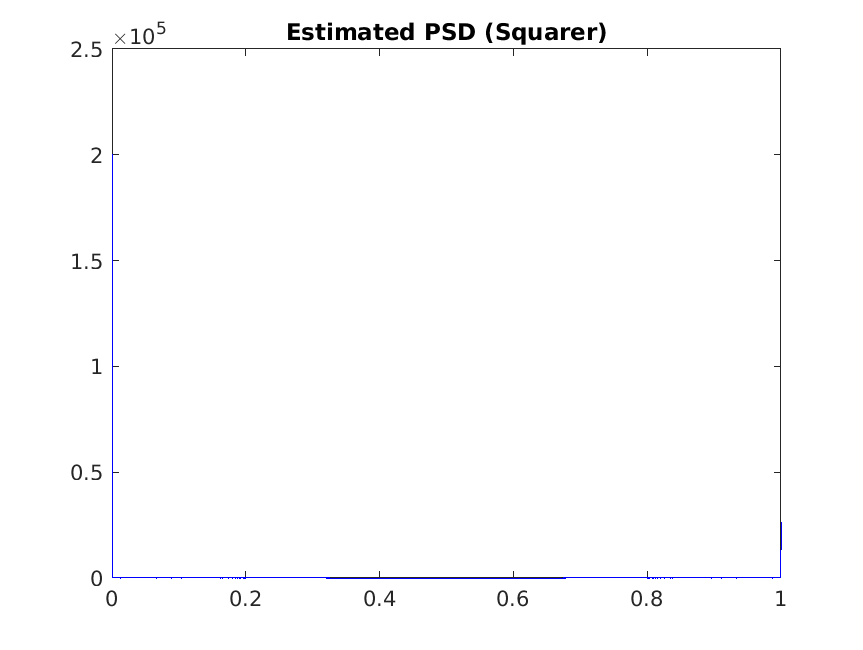
\includegraphics[width=0.6\textwidth]{images/study3/R_es_sq.png}
      \captionof{figure}{Estimated PSD}
    \end{center}
\end{figure}

Due to the non-linearity of the system, it has a peak in $f = 0$, so we can't
really see what's going on in the lower values of the y-axis. If we zoom, we
see something that looks more like the PSD we are looking for:

\begin{figure}[!hp]
    \begin{center}
      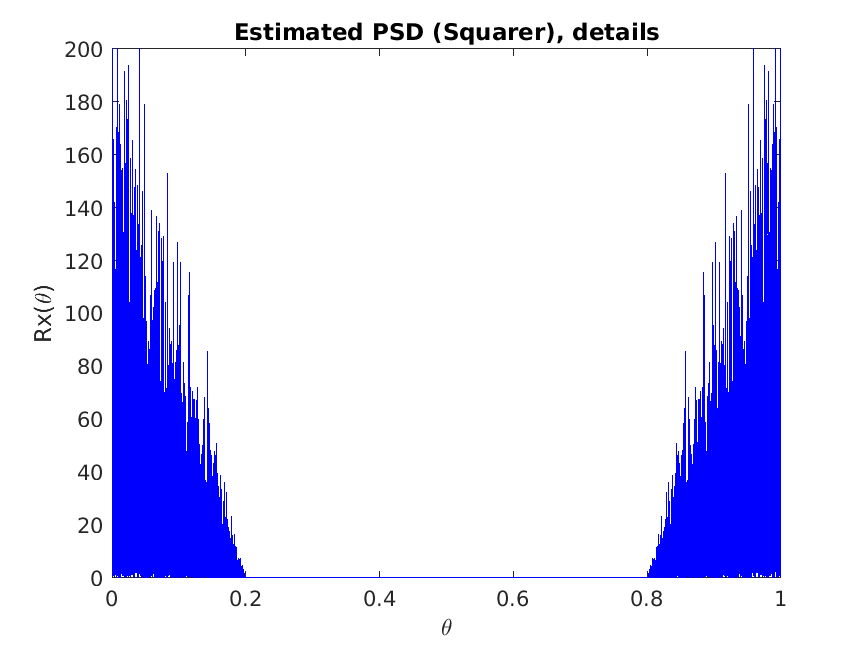
\includegraphics[width=0.6\textwidth]{images/study3/R_es_sq_zoom.png}
      \captionof{figure}{Zoomed Estimated PSD}
    \end{center}
\end{figure}

\newpage

We can compare it to the estimated PSD to see that, as every PSD we have seen
until now, it has a lot of variance, but we can see that it corresponds with
the function we already analyzed:

\begin{figure}[!hp]
    \begin{center}
      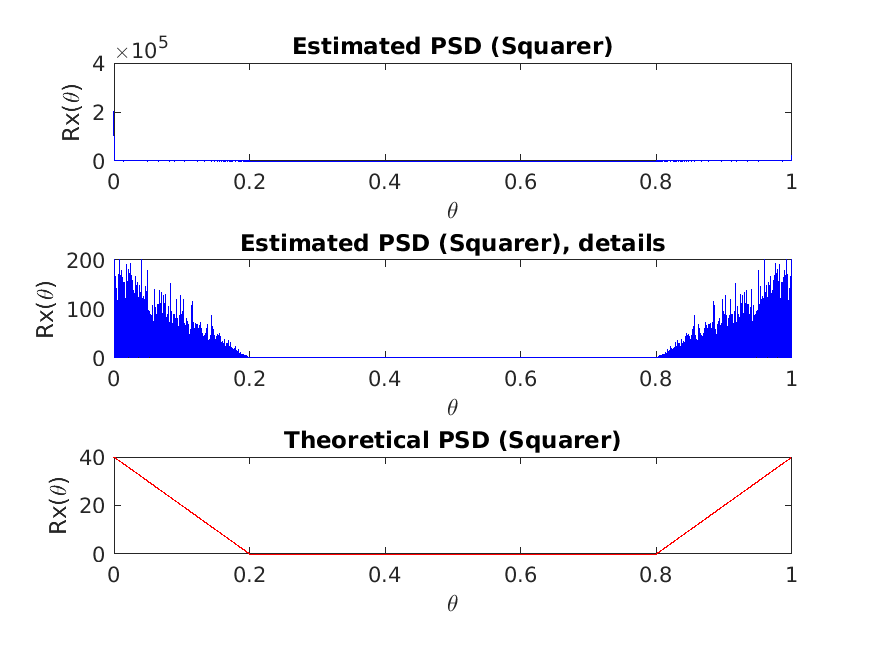
\includegraphics[width=0.6\textwidth]{images/study3/comp_psd_sq.png}
      \captionof{figure}{Compared PSD}
    \end{center}
\end{figure}

Lastly we can see the histogram of the squared signal:

\begin{figure}[!hp]
    \begin{center}
      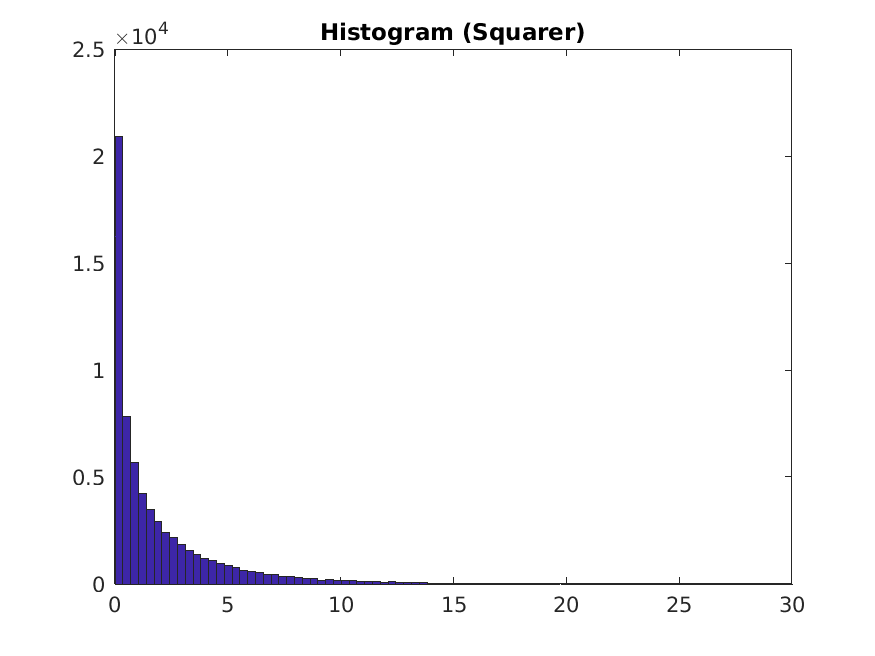
\includegraphics[width=0.6\textwidth]{images/study3/hist_sq.png}
      \captionof{figure}{Histogram}
    \end{center}
\end{figure}

We will analyze this in comparison to the initial filtered signal histogram
further on.

\newpage

\subsubsection{Half-Wave Rectifier:}

For the half-wave rectifier, we get this PSD estimation:

\begin{figure}[!hp]
    \begin{center}
      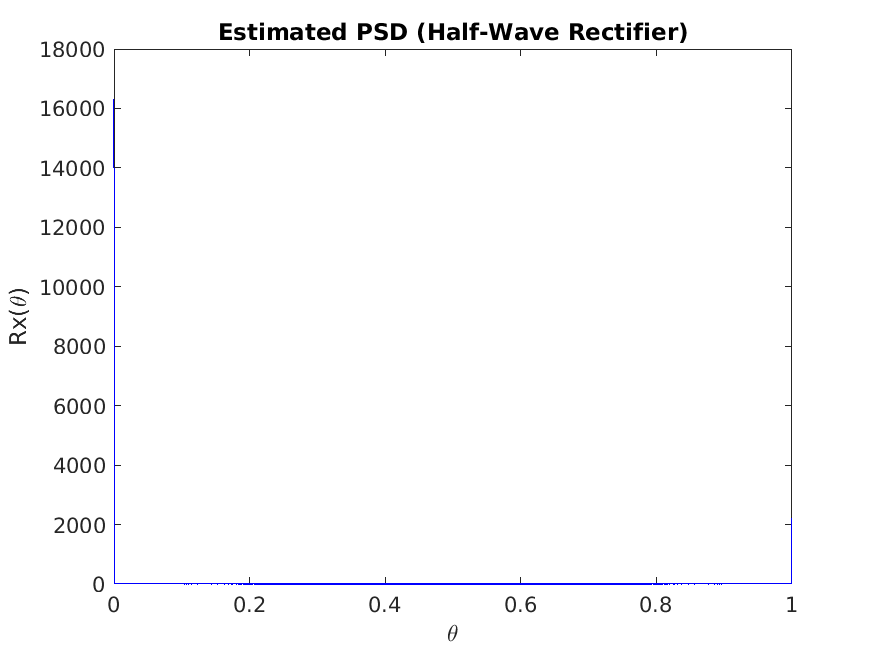
\includegraphics[width=0.62\textwidth]{images/study3/R_es_hw.png}
      \captionof{figure}{Estimated PSD}
    \end{center}
\end{figure}

Again, as the squarer PSD, it has a peak in $f = 0$. Therefore, we will zoom
the y-axis in the lower values to check:

\begin{figure}[!hp]
    \begin{center}
      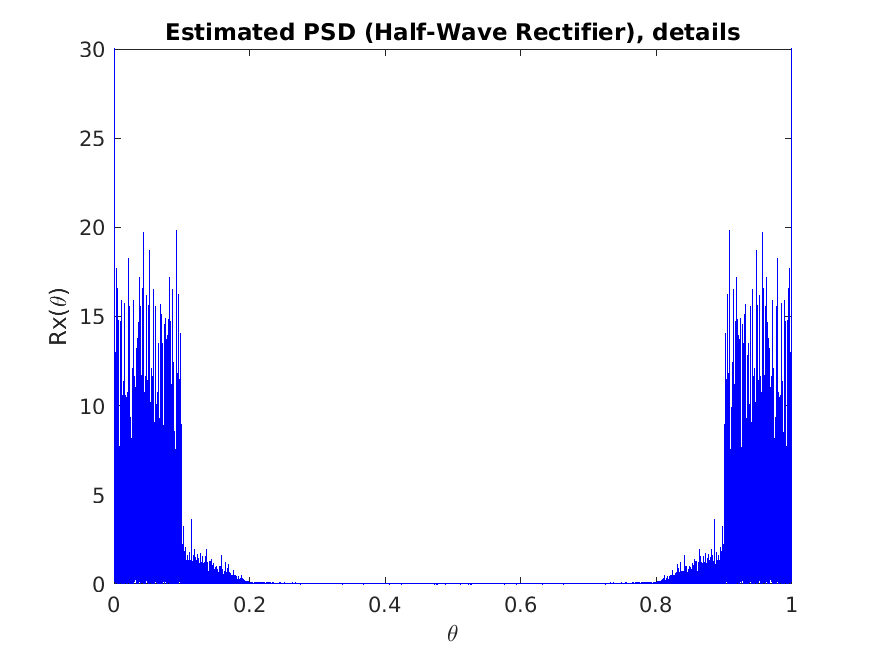
\includegraphics[width=0.62\textwidth]{images/study3/R_es_hw_zoom.png}
      \captionof{figure}{Zoomed Estimated PSD}
    \end{center}
\end{figure}

\newpage

We can compare it to the estimated PSD to see that, as every PSD we have seen
until now, it has a lot of variance, but we can see that it corresponds with
the function we already analyzed:

\begin{figure}[!hp]
    \begin{center}
      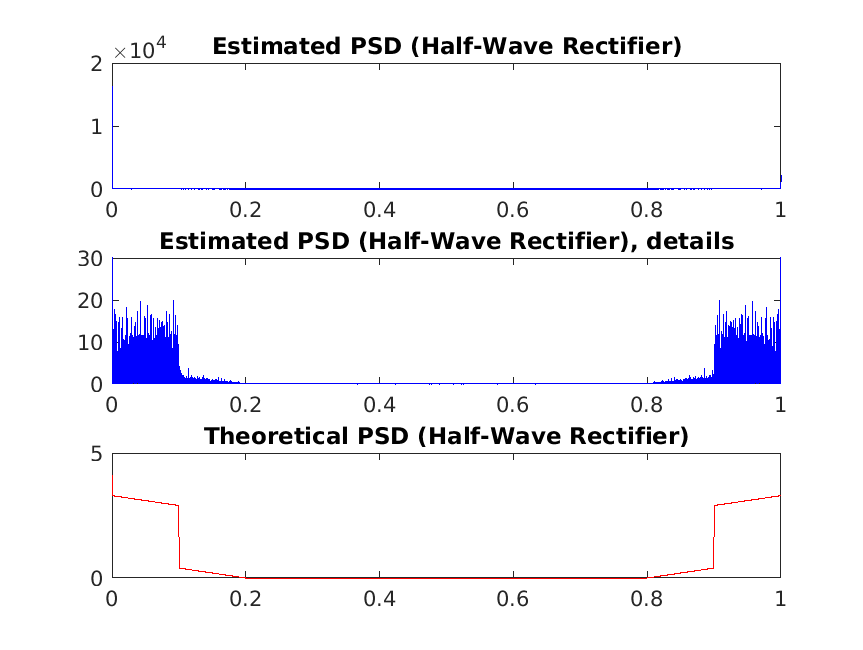
\includegraphics[width=0.6\textwidth]{images/study3/comp_psd_hw.png}
      \captionof{figure}{Compared PSD}
    \end{center}
\end{figure}

Lastly we can see the histogram of the rectified signal:

\begin{figure}[!hp]
    \begin{center}
      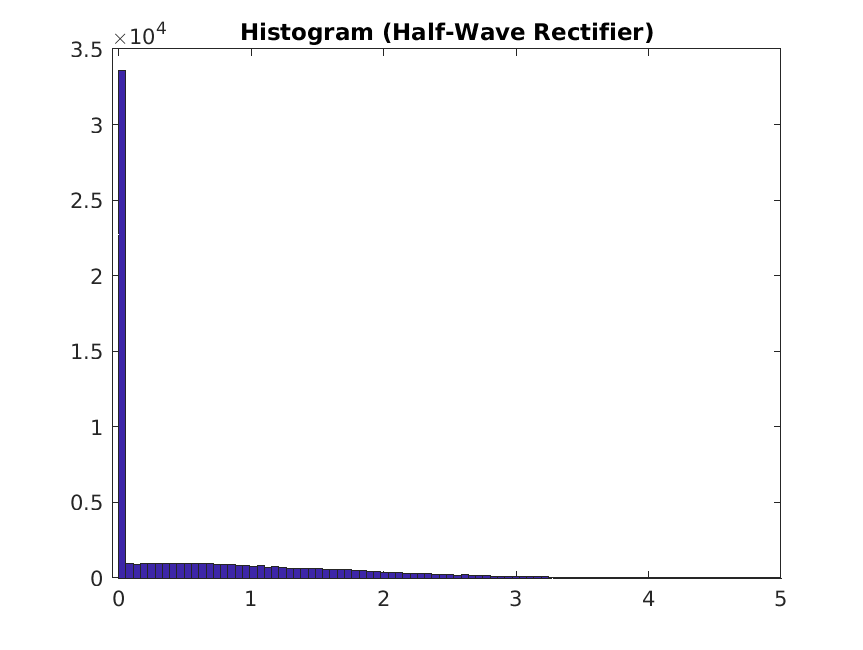
\includegraphics[width=0.6\textwidth]{images/study3/hist_hw.png}
      \captionof{figure}{Histogram}
    \end{center}
\end{figure}

\newpage

\subsubsection{AM-SC Modulator:}

For the AM-SC Modulator, we get this PSD estimation:

\begin{figure}[!hp]
    \begin{center}
      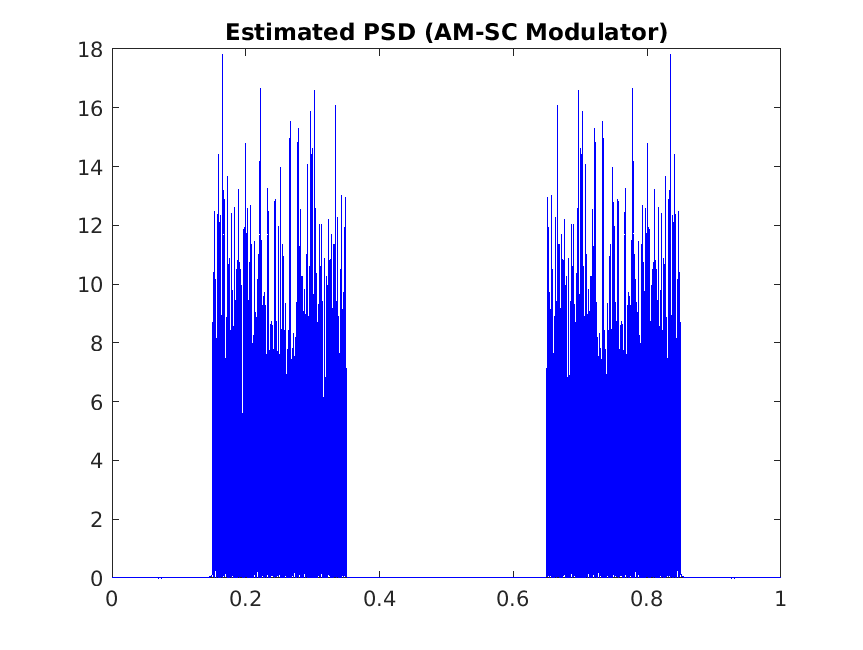
\includegraphics[width=0.62\textwidth]{images/study3/R_es_am.png}
      \captionof{figure}{Estimated PSD}
    \end{center}
\end{figure}

We can compare it to the estimated PSD to see that, as every PSD we have seen
until now, it has a lot of variance, but we can see that it corresponds with
the function we already analyzed:

\begin{figure}[!hp]
    \begin{center}
      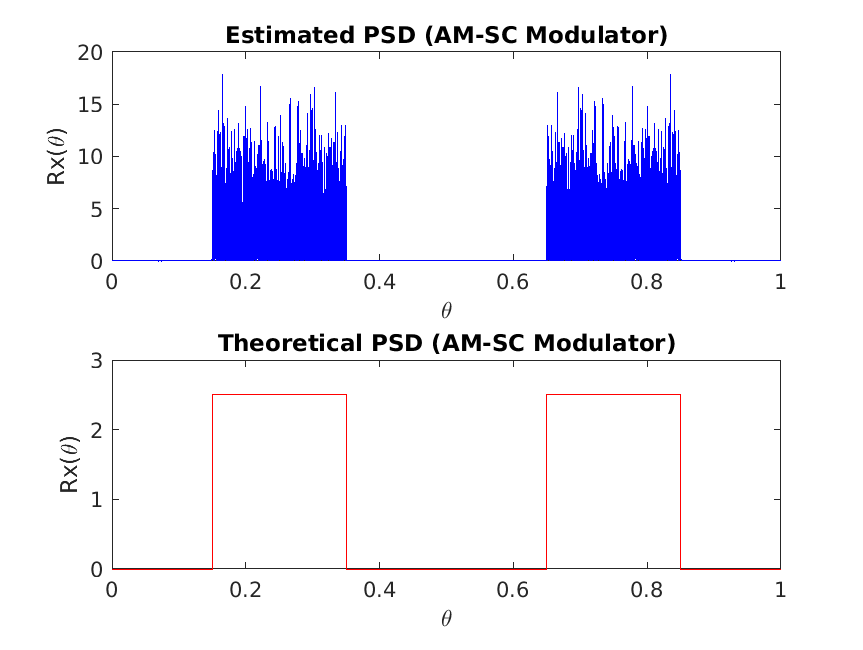
\includegraphics[width=0.62\textwidth]{images/study3/comp_psd_am.png}
      \captionof{figure}{Compared PSD}
    \end{center}
\end{figure}

\newpage

Lastly we can see the histogram of the modulated signal:

\begin{figure}[!hp]
    \begin{center}
      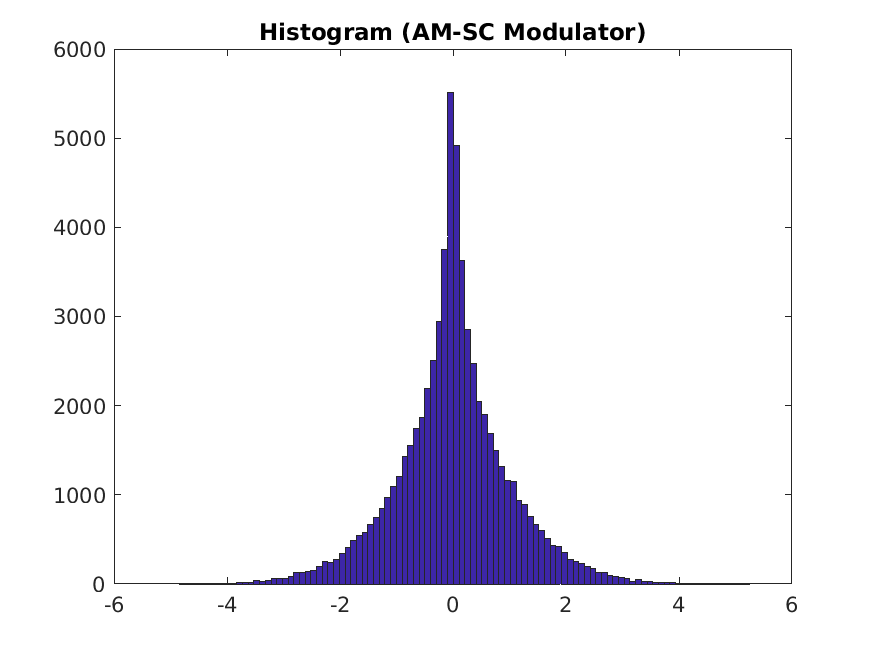
\includegraphics[width=0.6\textwidth]{images/study3/hist_am.png}
      \captionof{figure}{Histogram}
    \end{center}
\end{figure}

\subsection{Comparisons:}

Here we can see how the theoretical and estimated PSDs change depending on the
system we used and regarding the original filtered signal:

\begin{figure}[!hp]
    \begin{center}
      \includegraphics[width=0.65\textwidth]{images/study3/comp_psd_th.png}
      \captionof{figure}{Compared Theoretical PSDs}
    \end{center}
\end{figure}

\newpage

\begin{figure}[!hp]
    \begin{center}
      \includegraphics[width=0.7\textwidth]{images/study3/comp_psd_es.png}
      \captionof{figure}{Compared Estimated PSDs}
    \end{center}
\end{figure}

Here we can analyze the different histograms:

\begin{figure}[!hp]
    \begin{center}
      \includegraphics[width=0.7\textwidth]{images/study3/comp_hist.png}
      \captionof{figure}{Compared Histograms}
    \end{center}
\end{figure}

\newpage

For both the squarer and the half-wave rectifier, we get a peak near $f = 0$
in the estimated PSD that was not there in the original signal. Also, the PSD
is not zero from 0 to 0.2, and from 0.8 to 1 in both, which means that we have
PSD in frequencies different from the original PSD, that is, in more
frequencies than in the original PSD.
If we look at the histograms, the mean is no longer $0$, we only have positive
values and the shape of the curve is no longer Gaussian. Therefore, we can
conclude that the two first systems are non-linear.\\

For the AM-SC modulator, we have the same original PSD but moved in the x-axis
to the carrier frequency. Moving on to the histogram, we can see that it is
more similar to the original one than the other two histograms. The mean is
still $0$, and the values in which we have histogram are almost untouched, but
the Gaussian form is lost anyway. If the input was Gaussian and the output is
not Gaussian, we know that our system presents non-linearities, and therefore
out modulation has some non-linearities.\\

\newpage

\section{Study 4:}

\subsection{Theoretical Background:}

For this study we will be manipulating the signal in ways that are commonly
used in telecommunication areas.

We have two special operations:

\begin{equation}\label{eq:S1}
  Y[n] = X[n](-1)^n
\end{equation}

\begin{equation}
  Y[n] =
    \begin{cases}\label{eq:S2}
        X[n], & n: odd\\
        0,    & n: even\\
    \end{cases}
\end{equation}

Again, we will use our White Gaussian Noise and a high-degree low-pass filter
approximated as an ideal filter.

\subsection{Theoretical Analysis:}

\subsubsection{First System:}

Refering to formula \eqref{eq:S1}, we will have a system that takes our signal
and multiplies every value by either $+1$ or $-1$, alternating that sequence.

We have to calculate the PSD from the ACF:

\begin{equation}\label{eq:ACF_S1}
  \begin{split}
    & r_Y[k] = E\{Y[n+k]Y[n]\} =  E\{X[n+k]H[n+k]X[n]H[n]\} = \\
    & E\{X[n+k](-1)^{n+k}X[n](-1)^n\} = E\{X[n+k]X[n](-1)^{2n+k}\} = \\
    & E\{X[n+k]X[n](-1)^k\} = E\{X[n+k]X[n]\}(-1)^k = r_X[k](-1)^k
  \end{split}
\end{equation}

Now to go to the PSD we have to do the Fourier Transform of the above:

\begin{equation}\label{eq:R_hw}
  \begin{split}
    & \qquad\qquad R_Y[\theta] = \mathcal{F}\{r_Y[k]\} = \\
    & = \mathcal{F}\{r_X[k](-1)^k\} = R_X[\theta - 0.5] = \\
    & \qquad\qquad = R_X \text{rect}(\frac{\theta - 0.5}{BW})
  \end {split}
\end{equation}

\newpage

This is the result:

\begin{figure}[!hp]
    \begin{center}
      \includegraphics[width=0.9\textwidth]{images/study4/R_th_a.png}
      \captionof{figure}{Theoretical PSD}
    \end{center}
\end{figure}

\subsubsection{Second System:}

Refering to formula \eqref{eq:S2}, we will have a system that takes every other
value of our signal and multiplies it by 0, so we will have a sequence where
one every two values is 0 and the other is the actual value from out original
filtered signal. If we translate from formula \eqref{eq:S2} to a single-line
formula, we get:

\begin{equation}\label{eq:S2_2}
  Y[n] = \displaystyle\frac{1}{2}X[n](1-(-1)^{n+A})
\end{equation}

A is a random variable with $A \in [0,1]$ with the same probability of being 0
or 1, so in the end we decimate the signal. \\

Again, we have to calculate the PSD from the ACF:

\newpage

\begin{equation}\label{eq:ACF_S1}
  \begin{split}
    & \quad r_Y[k] = E\{Y[n+k]Y[n]\} =
    E\{\displaystyle\frac{1}{2}X[n+k](1-(-1)^{n+k+A})
    \displaystyle\frac{1}{2}X[n](1-(-1)^{n+A})\} = \\
    & = E\{X[n+k]X[n]\displaystyle\frac{1}{4}
    (1-(-1)^{n+k+A})(1-(-1)^{n+A})\} = \\
    & = \displaystyle\frac{1}{4}E\{X[n+k]X[n]
    (1-(-1)^{n+k+A}-(-1)^{n+A})+(-1)^{n+k+A+n+A})\} = \\
    & = \displaystyle\frac{1}{4}E\{X[n+k]X[n]
    (1-(-1)^{n+k+A}-(-1)^{n+A})+(-1)^{k})\} = \\
    & = \displaystyle\frac{1}{4}E\{X[n+k]X[n]
    (1-(-1)^{n+k+A}-(-1)^{n+A})+(-1)^{k})\} =  \\
    & = \displaystyle\frac{1}{4}[E\{X[n+k]X[n]\} - E\{X[n+k]X[n](-1)^{n+k+A}\} -
    E\{X[n+k]X[n](-1)^{n+A}\} + E\{X[n+k]X[n](-1)^{k}\}] =
    \displaystyle\frac{1}{4}[E\{X[n+k]X[n]\}  + E\{X[n+k]X[n](-1)^{k}\}] = \\
    & = \displaystyle\frac{1}{4}[E\{X[n+k]X[n]\}  + E\{X[n+k]X[n]\}(-1)^{k}] =
    \displaystyle\frac{1}{4}[r_X[k] + r_X[k](-1)^{k}]
  \end{split}
\end{equation}

Now to go to the PSD we have to do the Fourier Transform of the above:

\begin{equation}\label{eq:R_hw}
  \begin{split}
    & \qquad R_Y[\theta] = \mathcal{F}\{r_Y[k]\} =
    \mathcal{F}\{\displaystyle\frac{1}{4}[r_X[k] + r_X[k](-1)^{k}]\} = \\
    & = \displaystyle\frac{1}{4}(R_X[\theta - 0.5] + R_X[\theta]) =
    \displaystyle\frac{R_X}{4}(\text{rect}(\frac{\theta - 0.5}{BW}) +
    \text{rect}(\frac{\theta}{BW})
  \end{split}
\end{equation}

This is the result:

\begin{figure}[!hp]
    \begin{center}
      \includegraphics[width=0.7\textwidth]{images/study4/R_th_d.png}
      \captionof{figure}{Theoretical PSD}
    \end{center}
\end{figure}

\newpage

\subsection{Estimations:}

Now we will move to the estimatied PSDs:

\subsubsection{First System:}

For the first system we get this estimated PSD:

\begin{figure}[!hp]
    \begin{center}
      \includegraphics[width=0.6\textwidth]{images/study4/R_es_a.png}
      \captionof{figure}{Estimated PSD}
    \end{center}
\end{figure}

If we compare it to the theoretical PSD, we can see the similarities:

\begin{figure}[!hp]
    \begin{center}
      \includegraphics[width=0.6\textwidth]{images/study4/comp_psd_a.png}
      \captionof{figure}{Compared PSDs}
    \end{center}
\end{figure}

\newpage

\subsubsection{Second System:}

For the second system, the resulting graph is:

\begin{figure}[!hp]
    \begin{center}
      \includegraphics[width=0.65\textwidth]{images/study4/R_es_d.png}
      \captionof{figure}{Estimated PSD}
    \end{center}
\end{figure}

We can compare it to the theoretical PSD too:

\begin{figure}[!hp]
    \begin{center}
      \includegraphics[width=0.65\textwidth]{images/study4/comp_psd_d.png}
      \captionof{figure}{Compared PSDs}
    \end{center}
\end{figure}

\newpage

\subsection{Conclusions:}

\begin{figure}[!hp]
    \begin{center}
      \includegraphics[width=0.65\textwidth]{images/study4/comp_psd_th.png}
      \captionof{figure}{Compared Theoretical PSDs}
    \end{center}
\end{figure}

\begin{figure}[!hp]
    \begin{center}
      \includegraphics[width=0.65\textwidth]{images/study4/comp_psd_es.png}
      \captionof{figure}{Compared Estimated PSDs}
    \end{center}
\end{figure}

As we can see, in both systems we have the PSD in frequencies that we didn't
have in the input filtered signal. That mean that the systems are not LTI, like
the systems in study 3.

\vspace{4cm}

\end{document}
